%! TEX root = intro-optimization/main.tex
\chapter{Linear programming} % (fold)
\label{sec:Linear programming}
\section{General, standard form and augmented form linear programs} % (fold)
\label{sec:General, standard form and augmented form linear programs}

The most general form of a linear program is the following optimization problem.

\begin{align*}
  \min\, &f(x) = cx\\
  \text{s.t.}\, & Ax\ge b, x \in \mathbb{R}^{n}
.\end{align*}, for matrices \( A \in \mathbb{R}^{m \times n}\), row vector
\(c \in \mathbb{R}^{ 1\times  n} \).

\( m, n \) are called as the \textbf{number of variables} and the \textbf{number
of constraints} of the problem, respectively.

e.g. $\min f(x)=5x_{1}-6x_{2}+3x_{3}$ s.t. $8x_{1}+6x_{2}+6x_{3}=5$, $3x_{1}-2x_{2}+7x_{3}\geq 7$ and $x_{1},x_{2},x_{3}\geq 0$ has

\renewcommand\arraystretch{1.3}

\[
  [A|b]=\mleft[
  \begin{array}{ccc|c}
8 & 6 & 6 & 5 \\
-8 & -6 & -6 & -5 \\
3 & -2 & 7 & 7 \\
1 &  &  & 0 \\
 & 1 &  & 0 \\
	 &  & 1 & 0 \\
   \end{array}
   \mright], c=\begin{bmatrix}
5 & -6 & 3
\end{bmatrix}
\] (omited entries are \( 0 \))

As one can see, general form linear programs can model many different types of
constraints, like regular inequalities, equalities, and non-negative
requirements.

However, we will focus on solving a restricted form of the general problem, and
provide one a method to convert from any arbitrary general problem to a
restricted problem.

\begin{definition}
  A \textbf{standard form linear program} (SFLP) is an optimization problem in the
  form:
  \begin{align*}
  \min\, &f(x) = cx\\
  \text{s.t.}\, & Ax\ge b, x \ge  0
  .\end{align*}

  An \textbf{augmented form linear program} (AFLP) is an optimization problem in the
  form:
  \begin{align*}
  \min\, &f(x) = cx\\
  \text{s.t.}\, & Ax=  b, x \ge  0
  .\end{align*}
\end{definition}

To convert from the augmented form of a linear program to the standard form, one
can use the duplication trick as the above example, or even better, introduce a
new variable for each constraint. Such variables are called \textbf{slack
variables}.

\begin{align*}
  z &= \begin{bmatrix} x \\ y \end{bmatrix} \in \mathbb{R}^{n + m}\\
  A' &= \begin{bmatrix} A & I_{m} \end{bmatrix} \in \mathbb{R}^{m \times (n +
  m)}\\
    Ax \ge b &\iff y = b - Ax \ge  0\\
     &\iff  z \ge 0 \text{ and } Az = b
.\end{align*}, and
\begin{align*}
  &c' = \begin{bmatrix} c & 0_{m} \end{bmatrix} \in \mathbb{R}^{n + m}\\
  \implies f(x) &= cx = c'z = g(z)
.\end{align*}

Hence, the SFLP is equivalent to the following AFLP

  \begin{align*}
  \min\, &g(z) = c'z\\
  \text{s.t.}\, & A'z=  b, z \ge  0
  .\end{align*}

Converting from a general linear program to an SFLP is not as straightforward.
For every unbounded variables \( x^{i} \), let \( x^{i} = y^{i} - z^{i} \) for
some non-negative \( y^{i}, z^{i} \)
Then, the general problem is equivalent to the following SFLP

\begin{align*}
  \min\,&g(x') = c'x'\\
  \text{s.t.}\,& A'x' \ge  b, x' \ge  0
.\end{align*}, with 
\begin{align*}
  x' &= \begin{bmatrix} y \\ z \end{bmatrix} \in \mathbb{R}^{2n}\\
  A' & = \begin{bmatrix} A & -A \end{bmatrix} \in \mathbb{R}^{m \times  2n}\\
  c' &= \begin{bmatrix} c & -c \end{bmatrix} \in \mathbb{R}^{1 \times  2n} 
.\end{align*}.

Of course, this is the general case. In practice, one would want to minimize the
number of constraints and variables to make thing much easier to handle, by
utilizing "prebounded" and "already-slack" variables in the problem.
% section General, standard form and augmented form linear programs (end)

\section{Convex polyhedra} % (fold)
\label{sec:Convex polyhedra}

Let \( S \) be a subset of \( \mathbb{R}^{n} \). By convention, when we say "\(
S\) is open/closed/etc.", or talking about the boundary, closure, etc. of \( S
\), we refer to these topological concept with relative to the Euclidean
topology \( \mathbb{R}^{n} \). However, when one adds the \textit{relatively}
prefix, e.g. \( S \) is relatively open, without mentioning an explicit
topological space, that topological space is implicitly considered to be
generated from the metric space of \( \operatorname{aff} S  \), the
\textit{affine hull} of \( S \), equipped with the standard Euclidean norm.

For example, consider \( S = (-1, 1) \), then \( S \) is open (and not closed)
wrt \( \mathbb{R}
\), and both relatively open and closed wrt itself. However, since the affine
hull of \( S \) is \( \mathbb{R} \), we can not say that \( S \) is relatively
closed (without the "wrt" clause).

Consider the \( \mathbb{R}^3  \) space. The disk \( D = \{(x, y, 0), x^2+y^2\le
1\}   \), is closed wrt \( \mathbb{R}^3  \), but open in \( \mathbb{R}^2\times
\{0\}   \). The latter is the affine hull of \( D \), therefore we say that \( D
\) is relatively open.

It is trivial to see that relatively open/closed implies
open/closed, and the converse is not generally true. However, for closed
sets, this theorem holds.

\begin{theorem}
\label{thr:Relatively closed implies closed}
  If a set \( D \) is relatively closed, then \( D \) is closed.
  Hence, relatively closed and closed is the same thing.
\end{theorem}

For example, consider a hyperplane in higher dimensions. The hyperplane is
trivially relatively closed, since it is its own affine hull.

\begin{proof}
  Let \( A = \operatorname{aff} D \), \( D_{1} = A \setminus D, D_{2} =
  \mathbb{R}^{n} \setminus D \). We have \( D_{1} \subseteq D_{2} \) and \(
  A^{c} \subseteq D_{2} \).

  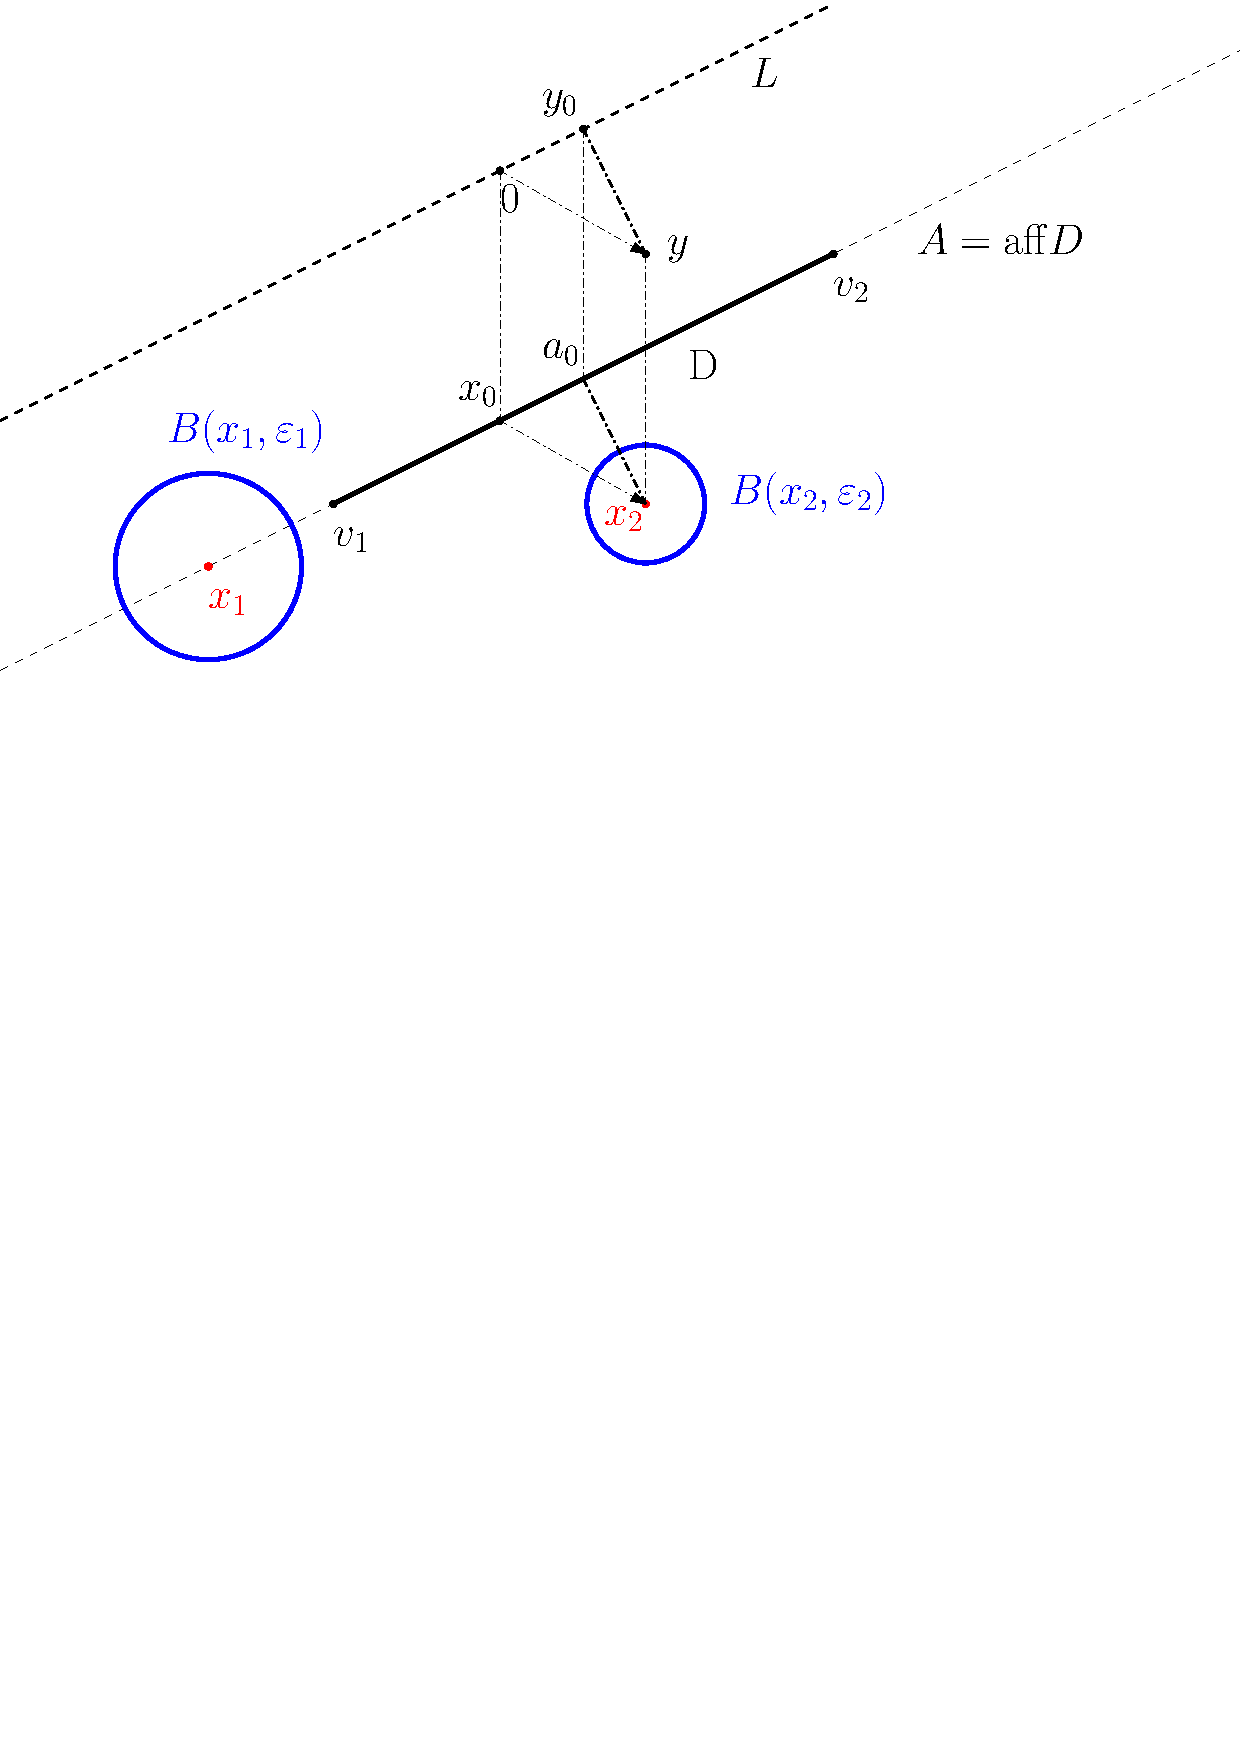
\includegraphics[scale=0.5]{figures/a}
  

  Then, \( D_{1} \) is relatively open. Let \( x \) be a point in \( D_{2} \).

  If \( x \in A \) (denoted as \( x_{1} \) in the figure above),
  then \( x \in A \). Then every neighborhood \( B_{A}(x,
  \varepsilon) \) of \( x \) is in \( D_{1} \), since \( D_{1} \) is open. Now
  consider \( y \in B(x, \varepsilon) \), then either \( y \in A \), implying \(
  y \in B_{A}(x, \varepsilon) \subseteq D_{1} \subseteq D_{2}\) or \( y \in
  A^{c} \subseteq D_{2} \). Hence, in all cases \( y \in D_{2} \), therefore \(
  B(x, \varepsilon) \subseteq D_{2}\).

  If \( x \in A^{c} \) (denoted as \( x_{2} \) in the figure above)
  and assuming \( A = x_{0} + L \) for some linear space \(
  L\). Then, we will prove that there exists \( \varepsilon > 0 \) such that \(
  d(x, a) < \varepsilon\) for all \( a \in A \). Intuitively, the distance from
  \( x \) to \( A \) is one such value for \( \varepsilon \).
  Making thing rigorous,
  let \( u = a - x_{0} \) and \( y = x - x_{0} \), then \( u \in L \). We will
  project \( x \) to \( A \), or equivalently, \( y \) to \( L \). Denote this
  projection as \( y_{0} \). Then, \( y \neq  y_{0} \) and \( d(y, y_{0}) > 0
  \). Pick \( \varepsilon = \frac{1}{2} d(y, y_{0}) \), then \( d(x, a) >
  \varepsilon \) , for every \( a \in A \), which means \( B(x, \varepsilon)
  \cap A = \varnothing \) or \( B(x, \varepsilon) \subseteq A^{c} \subseteq
  D_{2} \).

  In all cases, there exists \( \varepsilon > 0 \) such that \( B(x,
  \varepsilon) \in D_{2} \). Hence, \( D_{2} \) is open and \( D \) is closed.
\end{proof}



\subsection{Hyperplanes and related theorems} % (fold)
\label{sub:Hyperplanes and related theorems}

Consider the feasible for the above problem: \( D = \{x, Ax\ge b\}   \). Then,
one can see that \( D \) is the intersection of sets \( H_{i}=\{x, A^{i}x \ge
b^{i}\}   \) for \( i \) ranging from \( 1 \) to \( m \).

Now, we will have some names for these sets.

\begin{definition}
  A \textbf{hyperplane} is a set \( H \) in the form of \( H = \{x, ax =
  \alpha\}   \). \( H \) splits the whole space into two open sets, which are
  called \textbf{open half-spaces}: \( H_{1} = \{x, ax > b\}   \) and \( H_{2}
  = {x, ax < b} \). There are also \textbf{closed half spaces} \( H_{3} = H_{1}
  \cup H =
  \{x, ax \ge  b\}  \) and \( H_{4} = H_{2} \cup  H = \{x, ax \le  b\}   \). The
  vector \( a^{T} \) is a \textbf{normal} of \( H \).

  Let \( S \subseteq \mathbb{R}^{n} \) and \( x_{0} \in S \). Then, a hyperplane
  \( H = \{x, ax = \alpha\}   \) is a \textbf{supporting hyperplane} of \( S \)
  at \( x_{0} \) iff \( x_{0} \in H \) and either \( S \subseteq H_{1} \) or \(
  S \subseteq H_{2}\), with \( H_{1}, H_{2} \) being the closed half-spaces
  bounded by \( H \).

  Let \( A, B \) be two subsets of \( \mathbb{R}^{n} \). Then, a hyperplane \( H
  \) \textbf{separates} \( A \) and \( B \) if and only if \( H \) splits the \(
  \mathbb{R}^{n}\) space into two closed half-spaces \( H_{1} \) and \( H_{2} \)
  such that \( A \subseteq H_{1} \) and \( B \subseteq H_{2} \).
\end{definition}

Before going on proving the important hyperplane theorems, we start with a
simple lemma.

\begin{lemma}
\label{lem:Existence of closest element}
  Let \( S \) be a nonempty, closed set in \( \mathbb{R}^{n} \).
  Then for every \( x_{0} \in S^{c} \), there exists some \( x_{1} \in S \)
  such that \( d(x_{0}, x_{1}) \le d(x_{0}, x), \forall x \in S \).
\end{lemma}

\begin{proof}
  Note that this is basically a minimization problem: \( \min f(x) = d(x_{0}, x), x \in
  S\), then we can use the theorems in the last chapter to prove that a GOS
  exist. We will use Theorem \ref{thr:coercive condition}, which requires \(
  f(x) \) to be (lower semi-)continuous and \( \lim_{x \to \infty} f(x) =
  +\infty \), which are both basic properties of the Euclidean norm.
\end{proof}

\begin{theorem}[Hyperplane Separation Theorem (Closed set-point variant)]
\label{thr:hst-closed-pt}
  Let \( S \) be a nonempty, convex set and denote \( S' \) be its relative
  closure: \( S' = \operatorname{relclo} S = S \cup \operatorname{relbd} S \).
  Then for every \( x_{0} \in S'^{c} \),
  there exists some hyperplane separating \( S' \) (and therefore \( S \))
  and \( \{x_{0}\}   \). Moreover, we can construct a hyperplane that strictly
  separates \( S' \) and \( \{x_{0}\}   \).
\end{theorem}

\begin{proof}
  Let \( x_{1} \) be the closest point on \( \overline{S} \) to \( x_{0} \),
  denote \( d = (x_{1}-x_{0})^{T}\).

  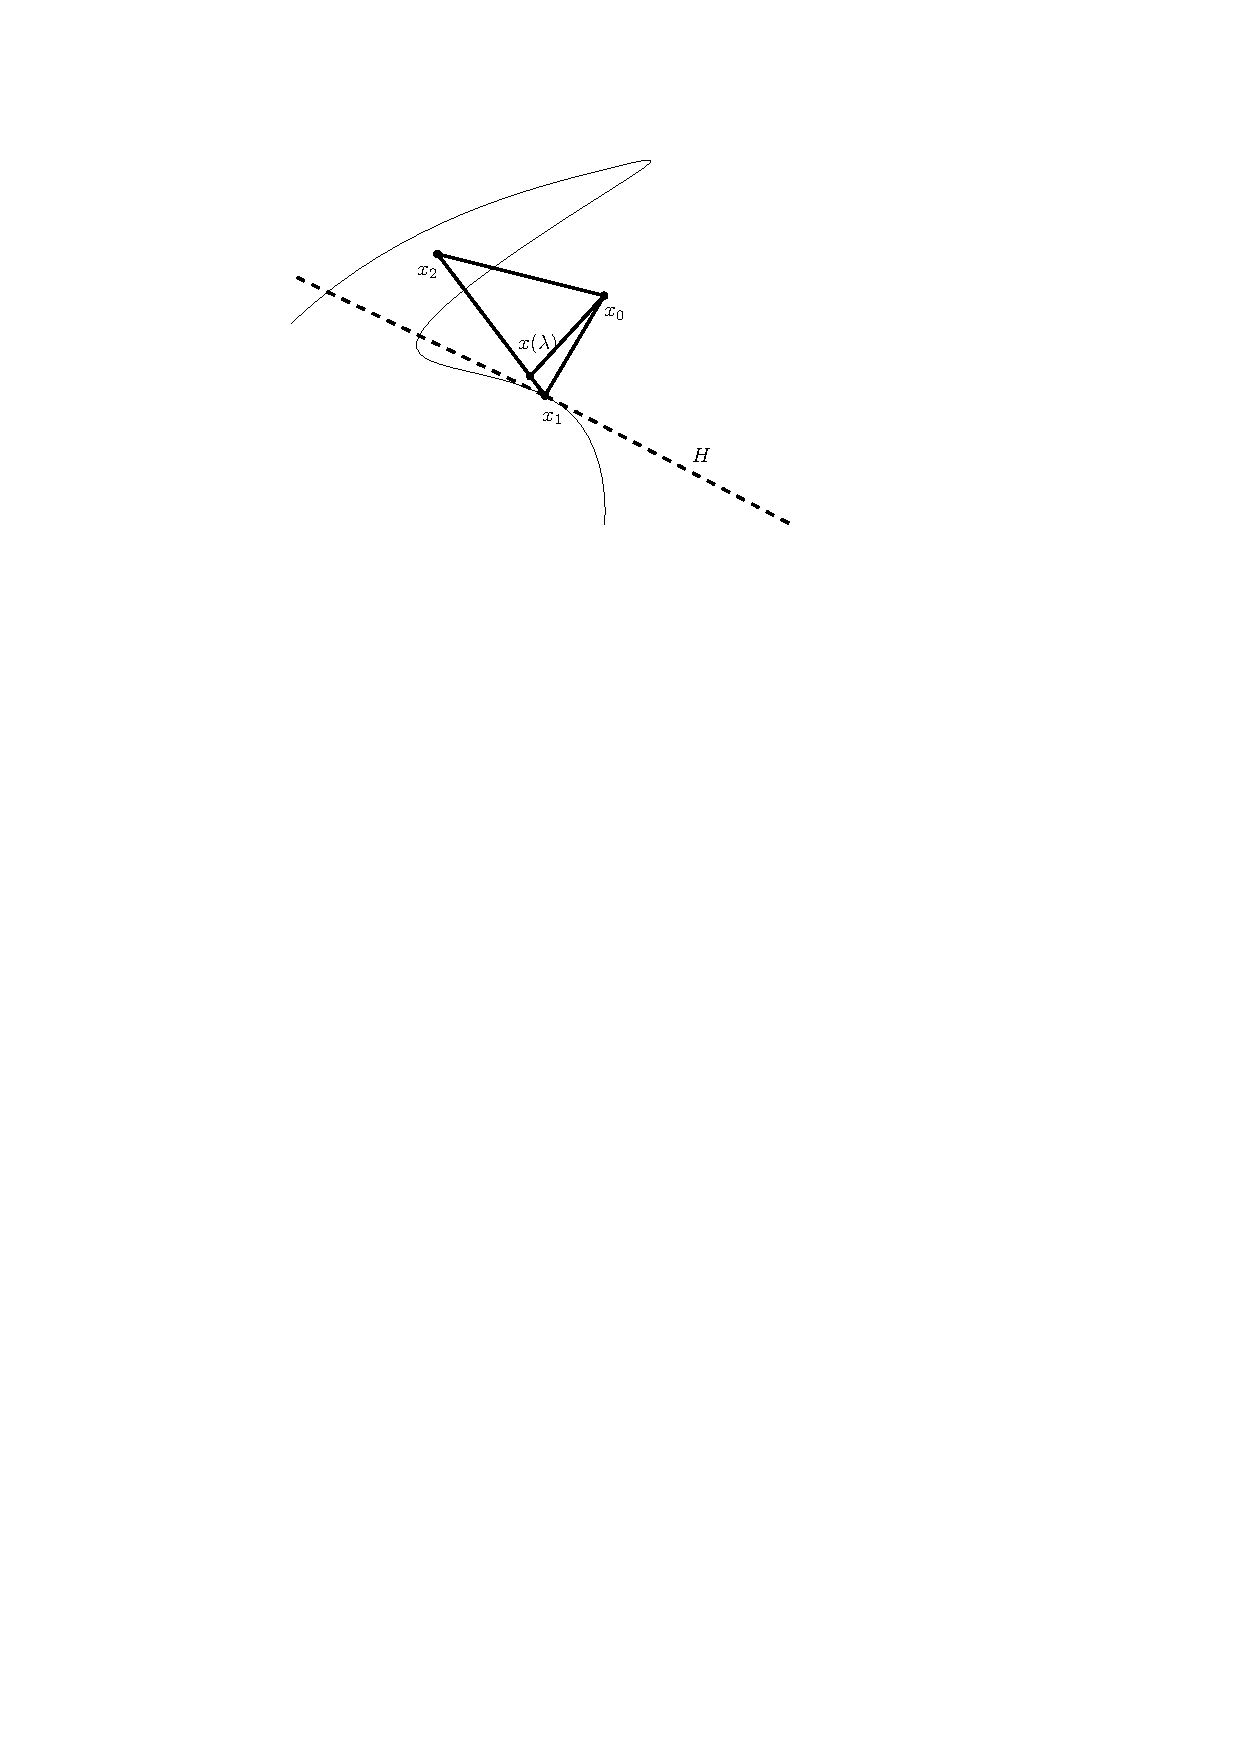
\includegraphics[scale=1.5]{figures/1696779691}

  Then, we will prove that the hyperplane \( H = \{x, dx = dx_{1}\}   \) is a
  supporting hyperplane of \( S \). If this is true, then it's trivial that \( H
  \) separates \( S \) and \( \{x_{0}\}   \).

  Now, we have \( dx_{0}-dx_{1}=-d^{T}d < 0 \), which means that \( x_{1} \in
  H_{1} = \{dx < dx_{1}\}   \). Hence, we need to prove that \( S \subseteq
  H_{2} = \{dx \ge  dx_{1}\}   \), or \( x \in S \implies dx \ge  dx_{1} \).

  Assuming that there is some \( x_{2} \in S \) such that \( dx_{2} < dx_{1} \).
  Consider the lerp between \( x_{2} \) and \( x_{1} \): \( x(\lambda) =
  \operatorname{lerp}(x_{2}, x_{1}, \lambda) \), which must be in \( S \) for
  every \( \lambda \in [0, 1] \)
  \begin{align*}
    x(\lambda) - x_{0} &= \operatorname{lerp}(x_{2}, x_{1}, \lambda) -
    x_{0}\\
                       &= \operatorname{lerp}(x_{2}-x_{1}, 0, \lambda) + (x_{1}
                       - x_{0})\\
                       &= \lambda(x_{2}-x_{1}) + d^{T}\\
  .\end{align*}

  \begin{align*}
    \|x(\lambda)-x_{0}\|^2 &= (\lambda(x_{2}-x_{1}) + d^{T})^{T}(\lambda(x_{2}-x_{1})
    + d^{T})\\
                           &= \|d\|^2 + 2\lambda d(x_{2}-x_{1}) + \lambda
                           ^2\|x_{2}-x_{1}\|^2\\
                           &= \|x_{1}-x_{0}\|^2 + \lambda g(\lambda)
  .\end{align*},
  with \( g(\lambda) = 2d(x_{2}-x_{1}) + \lambda \|x_{2}-x_{1}\|^2 < 0 \) for
  small \( \lambda > 0 \), which means that \( \lambda g(\lambda) < 0 \) and
  therefore \( x(\lambda) \) is closer to \( x_{0} \) than \( x_{1} \), which is
  a contradiction.

  To achieve strict separation, one take \( m = \frac{1}{2}(x_{0} + x_{1}) \),
  the midpoint of the \( [x_{0}, x_{1}] \) segment and construct a hyperplane \(
  H' \) parallel to \( H \), i.e. \( H': dx = \frac{1}{2}d(x_{0} + x_{1}) \),
  then we have \( dx_{0} > dm > dx, \forall  x \in A \), and therefore \( H' \)
  strictly separates \( S' \) and \( \{ x_{0}\}   \).
\end{proof}

\textbf{Remark. } The hyperplane \( H \) constructed above is a supporting
  hyperplane of \( S \) at \( x_{1} \).

\begin{corollary}
  A closed convex set \( S \) is the intersection of the closed half-spaces that
  contains \( S \).
\end{corollary}

\begin{proof}
  If \( x \in S \), then every closed half-space that contains \( S \) contains
  \( x \).

  If \( x \in S^{c} \), then there exists a supporting hyperplane separating \(
  S\) and \( \{x\}   \), which means that \( x \) could not be in the closed
  half-space that \( S \) is in.
\end{proof}


\begin{theorem}[Supporting Hyperplane Theorem]
  \label{thr:Supporting Hyperplane Theorem}
  Let \( S \) be a nonempty convex set and a point \( x_{0} \in \partial S \).
  Then, there exists a supporting hyperplane of \( S \) at \( x_{0} \).
\end{theorem}

\begin{proof}
  In every open ball \( B(x_{0}, \varepsilon_{n}) \), pick a point \( x_{n} \in
  B(x_{0}, \varepsilon_{n}) \cap  S^{c}\). Then, \( \lim_{n \to \infty} x_{n} =
  x_{0}\) if \( \varepsilon_{n} \to  0 \), which we will fix to \( \varepsilon_{n}
  = \frac{1}{n}\) for example.

  Using the previous theorem, there exists hyperplanes \( H_{n} \) separating \(
  S\) from \( \{x_{n}\}   \). Let the normal unit vector of \( H_{n} \) be \(
  d_{n} \), with the convention that \( d_{n}(x-x_{n}) \ge 0, \forall  x \in
  S \).

  Hence, \( d_{n} \) is a sequence on the compact set \( \partial B(0, 1) \),
  which means that there must be a convergent subsequence \( d_{i_{n}} \) that
  converges to \( d \).

  Since \( d_{n}(x-x_{n}) \ge 0 \) for all \( x \in S \), letting \( n = i_{m}
  \) and \( m \to  \infty \), we have \( d(x-x_{0}) \ge 0 \), and therefore \(
  H=\{x, d(x-x_{0})\ge 0\}   \) is a supporting hyperplane of \( S \).
\end{proof}

\textbf{Remark. } This result also holds for all \( x_{0} \in
\operatorname{relbd} S
\), since \( \operatorname{relbd} S \subseteq \partial S \).

\begin{corollary}[Hyperplane Separation Theorem (Set-point variant)]
\label{cor:hst-set-pt}
  Let \( S \) be a nonempty convex set, then for every \( x \in
  (\operatorname{Int} S)^{c} \), there is a supporting hyperplane \( H \) that
  separates \( S \) and \( \{ x\}   \).
\end{corollary}

\begin{proof}
  If \( x \in \partial S \), the supporting hyperplane exists due to Theorem
  \ref{thr:Supporting Hyperplane Theorem}.

  If \( x \in \overline{S}^{c} \), then if \(\overline{S} \) is a convex set,
  there exists a supporting hyperplane of \( \overline{S} \) at \( x \), which
  is also a supporting hyperplane of \( S \) at \( x \), due to Theorem
  \ref{thr:hst-closed-pt}.

  To conclude, one would need to prove that \( \overline{S} \) is convex, using
  the following argument:

    \( \overline{S} \) is the set of all \( x \) such that there exists a
    sequence \( (x_{n})_{n \in \mathbb{N}} \), \( x_{n} \in S, \forall n \in
    \mathbb{N} \) converges to \( x \).

    Consider a point tuple \( A = (A^{1}, A^{2}, \ldots , A^{m}), A^{i} \in
    \overline{S}, \forall i \in 1..m \). To prove \( \overline{S}
    \) is convex, we need to prove that \( x = \mathcal{C}(A, \lambda) \in
    \overline{S} \), for
    all \( \lambda \in \mathbb{R}^{m} \) satisfying the convex conditions.

    Let \( (A_{n})_{n \in \mathbb{N}} \) be the sequence that converges to \( A
    \). Then, \( x_{n} = \mathcal{C}(A_{n}, \lambda) \to  \mathcal{C}(A, \lambda) =
    x\) because of linearity, as \( n \to  \infty \). Note that \( x_{n} \in S
    \) and therefore \( x \in \overline{S} \).
\end{proof}

Finally, we can prove the \textbf{Hyperplane separation theorem}.
\begin{theorem}[Hyperplane Separation Theorem]
\label{thr:Hyperplane Separation Theorem}
  Let \( A, B \) be nonempty disjoint convex sets, then there exists a
  hyperplane that separates the sets.
\end{theorem}

\begin{proof}
  Consider the set \( S = S_{1} - S_{2} = \{s_{1} - s_{2},
  s_{1} \in S_{1}, s_{2} \in S_{2}\}   \).

  \( S \) is convex, since if \( x_{1}-x_{2}, y_{1}-y_{2} \in S_{1}-S_{2} \)
  (s.t. \( x_{1},y_{1} \in S_{1}, x_{2}, y_{2} \in S_{2} \)), then a convex
  combination of the two, which can be written as \(
  \operatorname{lerp}(x_{1}-x_{2},y_{1}-y_{2},\lambda) =
  \operatorname{lerp}(x_{1},y_{1},\lambda) -
  \operatorname{lerp}(x_{2},y_{2},\lambda) \in S_{1}-S_{2} \) due to the fact
  that \( \operatorname{lerp}(x_{i},y_{i}, \lambda) \in S_{i} \).

  Then, using Corollary \ref{cor:hst-set-pt}, there is a hyperplane separating
  \( S_{1}-S_{2} \) and \( \{0\}   \). Moreover, there is one such hyperplane
  that passes through \( 0 \), which could be constructed by slightly modifying
  the proofs of the above theorems. Denote this hyperplane as \( H = \{x, dx \ge
  0\}   \), then we have \( dx_{1} \ge  dx_{2}, \forall x_{1} \in S_{1}, x_{2}
  \in S_{2} \).

  Let \( \alpha = \inf dS_{1}, \beta = \sup dS_{2} \), then we have \( dx_{1}
  \ge  \alpha \ge  \beta \ge dx_{2}, \forall x_{1} \in S_{1},x_{2} \in S_{2} \),
  which yields at least one separating hyperplane of \( S_{1} \) and \( S_{2}
  \): \( H'(\gamma) = \{ dx = \gamma\}   \) for any \( \gamma \in [\alpha,\beta]
  \), which is a nonempty interval.
\end{proof}

% subsection Hyperplanes and related theorems (end)

\subsection{Extreme points and recession directions} % (fold)
\label{sub:Extreme points and recession directions}

\begin{definition}
  Let \( S \) be a subset of \( \mathbb{R}^{n} \).

  If \( S \) is convex, then \( x \in S \) is an \textbf{extreme point} if and only if
  it could not be written as a strictly convex combination of a collection
  of points in
  \( S \) not containing \( x \). In other words, \( x \in S \) is an extreme
  point if for every \( y, z \in S \setminus \{x\}, w \in (0, 1)   \), we have
  \( x \neq \operatorname{lerp}(y,z,w) \).

  If a vector \( v \) satisfies, \( x + tv \in S \) for every \( x \in S \), \(
  t \ge  0\), then \( v \) is a \textbf{recession direction} of \( S \).

  A recession direction \( v \) is called a \textbf{extreme direction} if it is
  not a strictly convex combination of any collection of recession directions
  not containing directions in the form \( kv \) for scalars \( k \in \mathbb{R}
  \).
\end{definition}

Before going on proving the  \textbf{Krein-Milman Theorem}, we will look at
\textbf{faces}.

\begin{definition}
  Let \( S \) be a closed convex set. Then a convex \( F \subseteq S \)
  is a \textbf{face} iff \( \forall A \subseteq S \),
  \( \exists x \in F \) is a \textit{strict convex combination} of
  finite \( A \), then \( A \subseteq F \).

  If \( F \neq S \), then \( F \) is called a \textbf{proper face} of \( S \).
\end{definition}

By this definition, any closed, convex set \( S \) is its own face.
Additionally, the empty set \( \varnothing \) is also a face of every closed,
convex set \( S \). These are called as improper faces. The remaining faces,
i.e. faces of \( S \) that is not \( \varnothing \) or \( S \), are
\textbf{proper faces} of \( S \).

\begin{theorem}
\label{thr:No proper faces with full dimensions}
  Let \( S \) be a nonempty closed convex set with \( n = \dim S
  \). Then, if \( F \) is a face with \( n = \dim F \), \( F = S
  \).
\end{theorem}

\begin{proof}
  The idea of the proof goes as follows.
  Assuming \( F \neq  S \), \( F \) is a face of \( S \) and \(
  \dim F = \operatorname{dim} S = n \). Then, take \( x \in S
  \setminus F \) and let \( X \) be a maximum set of affinely independent points
  in \( F \),
  then \( n = \dim F = |X| \).
  If \( X' = X \cup \{x\} \subseteq S   \) is affinely independent, then \( |X'|
  = |X| + 1 = \dim S = n \). This means that \( n = n + 1 \),
  which is a contradiction.

  Hence, \( X' \) could not be affinely independent, which means that \( x \) is
  in the affine hull of \( X \), which will be denoted as \( A \). Note that \(
  F \subseteq \operatorname{aff} X\), hence \( F \subseteq A \).

  Pick a point \( x' \in \operatorname{ri} F \) (we will prove that \(
  \operatorname{ri} F \) is nonempty later), then for small enough \( \lambda
  \), \( x_{0} = \operatorname{lerp}(x', x, \lambda) \) will reside in the open ball \(
  B_{A}(x', \varepsilon) \subseteq F\). Hence, the segment \( [x', x] \)
  intersects \( F \) at \( x_{0} \in F \), which means \( x', x \in F \), which
  contradicts with the face that \( x \in S \setminus F \).

  Finally, we need to prove that \( \operatorname{ri} F \) is nonempty. This
  follows from the following lemma.

  \begin{lemma}
  \label{lem:Nonempty convex set has nonempty interior}
    Every nonempty convex set \( C \) has nonempty interior \( \operatorname{ri}
    C \neq  \varnothing \)
  \end{lemma}

  \begin{proof}[Proof of lemma]
  WLOG, translate \( C \) such that \( 0 \in C \). Then, pick \( n \)
  affinely independent vectors in \( C \) (this is possible since \( n =
  \dim S \)), denoted as \( b_{1}, b_{2}, \ldots , b_{n} \). This
  can be collected into a matrix \( b \), and the representing linear map \(
  f(x) = bx \) will map \( \mathcal{S} = \operatorname{conv} \{0, \mathbf{e_{1}},
  \mathbf{e_{2}}, \ldots, \mathbf{e_{n}} \}   \) to \( \operatorname{conv} \{0,
  b_{1}, b_{2}, \ldots , b_{n}\} \subseteq C   \). This map preserves (relatively)
  interior points, and the set \( \mathcal{S} \) trivially have a nonempty interior,
  therefore \( C \) must have at least an interior point.
  \end{proof}
\end{proof}

Aside from the nonproper faces, there is also a class of faces that is very
special.

\begin{theorem}
\label{thr:Every extreme point forms a face}
  Let \( S \) be a convex set. Then, for \( x_{0} \in S \) is an extreme point
  if and only if \( F = \{x_{0}\}   \) is a face of \( S \).
\end{theorem}

\begin{proof}
  This trivially follows from the definition of extreme points and faces.

  \( x_{0} \) is an extreme point of \( S \) iff it could not be written as a
  strictly convex combination of points in \( S \ \{ x_{0} \} = S \setminus F
  \). Since \( F \) only contains \( x_{0} \), this is equivalent to the fact
  that \( F \) is a face of \( S \).
\end{proof}


\begin{theorem}
  If \( F \) is a face of a closed, convex set \( S \), then \( F \) is also
  closed. Moreover, all faces of \( F \) are faces of \( S \).
\end{theorem}

\begin{proof}
  For nonproper faces \( F \), the theorem is trivial. We will only consider
  proper faces \( F \).

  \centerline{
    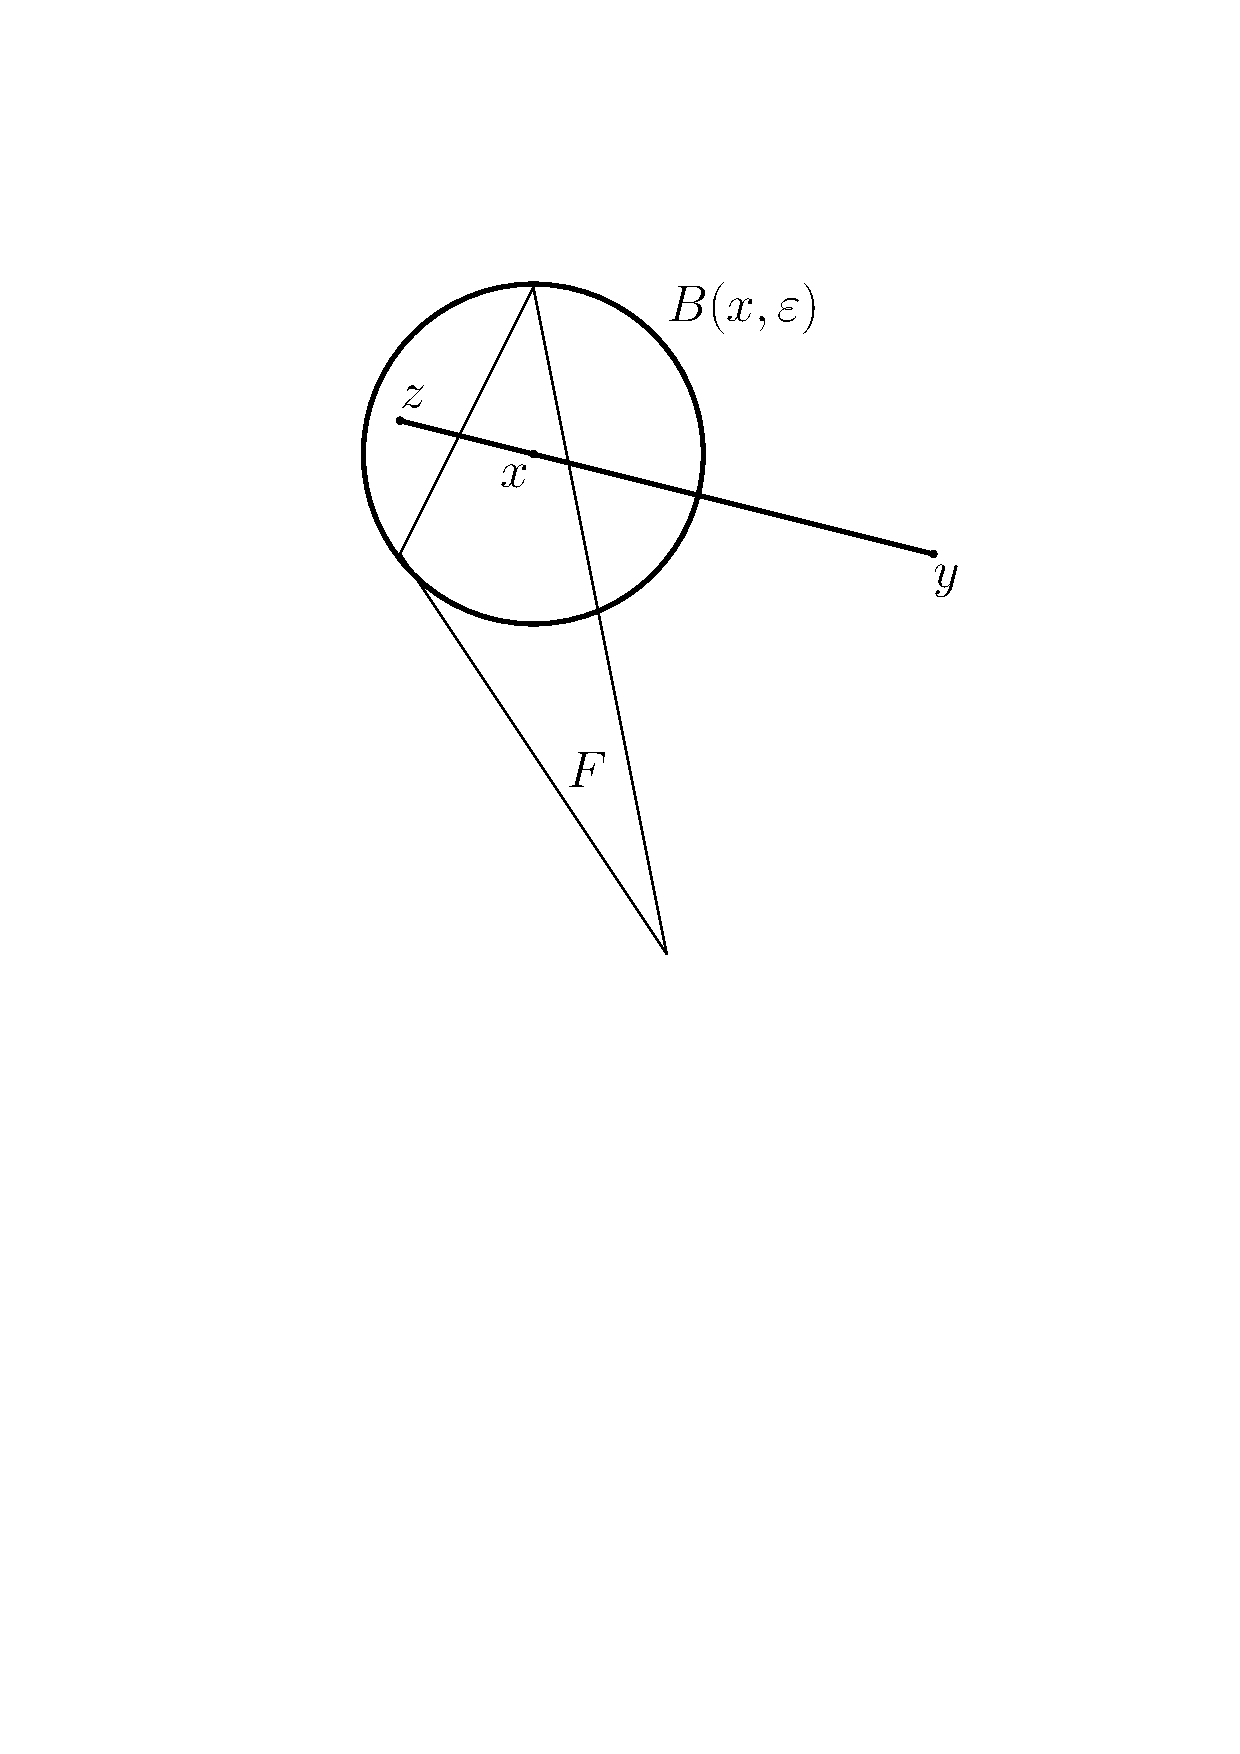
\includegraphics[scale=0.5]{figures/1696828548}
  }

  Since relatively closed and closed are the same thing, the relative closure of
  a set is simply its closure. Hence, there is no need to differentiate between
  the relative closure of \( F \) and \( \overline{F} \). Another important
  thing to note is that \( \overline{F} \subseteq S \), because of the
  minimality of closures.

  Using Lemma \ref{lem:Nonempty convex set has nonempty interior}, we have proven
  that every nonempty convex set has a nonempty interior. Pick \( x \in
  \operatorname{ri} F \), then for all \( y \in \overline{F}
  \setminus \{ x\}   \), and consider the ray \( R = \{x + \lambda (y - x),
  \lambda \ge  0\}   \).

  Consider the intersection \( I \) of the ray with \( \overline{F} \). Since \(
  \overline{F}\) and \( R \) are closed, \( I \) must be closed and convex, \( I
  \) is also a closed and convex set.

  Consider the set \( L = \{ \lambda \ge 0, x + \lambda(y - x) \in
  \overline{F}\}   \). This set is nonempty (\( 0 \in L \)), and therefore has
  a supremum \( \lambda_{0} = \sup L \ge 0 \). Then, there exists a
  diffeomorphism between \( L \) and \( I \): \( f(\lambda) = x + \lambda(y - x)
  \), and therefore \( L \) is convex and closed. Hence, it is trivial to prove
  that \( L \) contains the segment \( [0, \lambda_{0}] \) and because of the
  maximality of \( \lambda_{0} \), \( L = [0, \lambda_{0}] \).

  We have two cases.
  \begin{itemize}
  \item If \( \lambda_{0} = 0 \), then \( L = \{0\}   \). Then every point \(
    z_{\lambda}
    = x + \lambda(y - x) \notin \overline{F}\). For every neighborhood \( B(x,
    \varepsilon) \)
    of \( x_{0} \) with relative to \( A = \operatorname{aff} F \), there exists
    \( z_{\varepsilon} \in B(x, \varepsilon) \) not in \( \overline{F} \) and \(
    z_{-\varepsilon} \in [x, y] \subseteq \overline{F} \), for arbitrarily small
    \( \varepsilon > 0 \). Then, \( x \in \operatorname{relbd} F \), which is a
    contradiction with \( x \in \operatorname{ri} F \).
  \item If \( s > 0 \), then \( x \) is a strictly convex combination of \( y \)
    and \( z = x + s(y - x) \). Then, \( y, z \in F \) due to the definition of
    faces.
  \end{itemize}

  Hence, \( y \in F \) for every \( y \in \overline{F} \), which means \(
  \overline{F} \subseteq F \), or \( F = \overline{F} \) is a closed set.

  \iffalse
  \begin{itemize}
    \item Let \( A \subseteq S \) be a finite set such that \( x =
      \mathcal{C}(A, \lambda) \in S \), then \( A \subseteq F \) because of the
      definition of faces. Using the definition once more for \( F' \), we have
      \( A \subseteq F' \), which means \( F' \) is a face of \( S \).


    \item 
    \item Pick \( x \in F \) (if \( F = \varnothing \) then \( F \) is easily
      closed). Let \( L \) be the linear space that is parallel to \(
      \operatorname{relclo} F = F \cup \operatorname{relbd} F \), the relative
      closure of \( F \), since \( x, y \in F \) we have \( y - x \in L \).
      Then, one can pick \( z = x + \lambda(x - y) \) for some \( \lambda \ge 0
      \) such that \( z \in B(x, \varepsilon) \subseteq \operatorname{^{i} } F
      \), which means \( x \) is now a strict convex combination of \( y \) and
      \( z \). Since \( F \) is a face, \( y, z \in F \). Hence, \(
      \operatorname{relclo} F = F \), which means that \( F \) is closed.

      To make the proof more rigorous, we need to prove \( \operatorname{relclo}
      F \subseteq S\), which comes from \( S \) being a closed convex set. This
      is a rather trivial result, coming from the fact that the closure of a set
      \( F \) is the minimal closed set containing \( F \).
  \end{itemize}
  \fi
\end{proof}

\textbf{Remark.} The condition \( F \) convex in the definition of a face is very
important, without it the above theorem fails to hold.

For example, take \( S = \{(x, y), x^2 + y^2 \le  1\}   \), the closed unit
circle. This set is convex, closed and bounded. The upper-half circle, denoted
as \( U = \{(x, y) \in S, x^2 + y^2 = 1, y > 0\}     \) is a "face" of \( S \)
(if convexity is not needed for faces), but it is not closed. This is due to \(
\operatorname{ri} F = \varnothing\), breaking down the whole proof above.

Consider a face \( F' \) of a face \( F \) of \( S \). If \( x \in F' \), then
every strictly convex combination \( x = \mathcal{C}(A, \lambda), A \subseteq
F\), implies that \( A \subseteq F' \). Moreover, since \( x \in F \), the
condition \( x = \mathcal{C}(A, \lambda), A \subseteq S \) implies \( A
\subseteq F \). Hence, for every strictly convex combination \( x =
\mathcal{C}(A, \lambda), A \subseteq S \), we can deduce that \( A \subseteq F'
\). In other words, \textbf{faces of faces are also faces of the set}.

Since extreme points form a special class of faces, we also have a corollary of
this fact: \textbf{extreme points of faces are also extreme points of the set}.

Hence, we have the following theorem.

\begin{theorem}[Faces and extreme points of faces]
\label{thr:Faces and extreme points of faces}
  Let \( F \) be a face of a convex set \( S \). Then:
  \begin{itemize}
  \item Every face \( F' \) of \( F \) is a face of \( S \).
  \item Every extreme point \( x_{0} \) of \( F \) is an extreme point of \( S
    \).
  \end{itemize}
\end{theorem}

Now, we will look at a class of faces that will be very important for our
purposes.

\begin{theorem}[Exposed faces]
\label{thr:Exposed faces}
  Let \( C \) be a convex set that lies on one closed half-space of the
  hyperplane \( H: ax = \alpha \). Then, the intersection of \( C \) and \( H
  \), \( F = C \cap H = \{x \in C, ax = \alpha\}   \), called an \textbf{exposed
  face induced by} \( H \), is a face.
\end{theorem}

\begin{proof}
  Assuming \( C \subseteq H' = \{x \in \mathbb{R}^{n}, ax \le  \alpha\}   \).
  Then assuming \( \exists y, z \in C \) such that \( \operatorname{lerp}(y, z,
  \lambda) \in F \) for some \( \lambda \in (0, 1) \) and \( y \neq  z \).

  Now,
  \begin{align*}
    \operatorname{lerp}(y, z, \lambda) \in F &\iff a\operatorname{lerp}(y, z,
    \lambda)\\
                                             &\iff \operatorname{lerp}(ay, az,
                                             \lambda) = \alpha
  .\end{align*}
  
  Since \( y, z \in C \), \( ay, az \le \alpha \). Then, \(
  \operatorname{lerp}(ay, az, \lambda) \le \alpha \) for some \( \lambda \in (0,
  1) \). Equality occurs if and only if \( ay = az = \alpha \), which means \(
  y, z \in F \). Hence, \( F \) is a face.
\end{proof}

This theorem gives us a way to find a whole class of faces of an arbitrary
(most optimally compact) convex set in an intuitive sense. Simply move a
hyperplane along its normal until it hit the set, and then the intersection
would be a face of the convex set.
\newpage

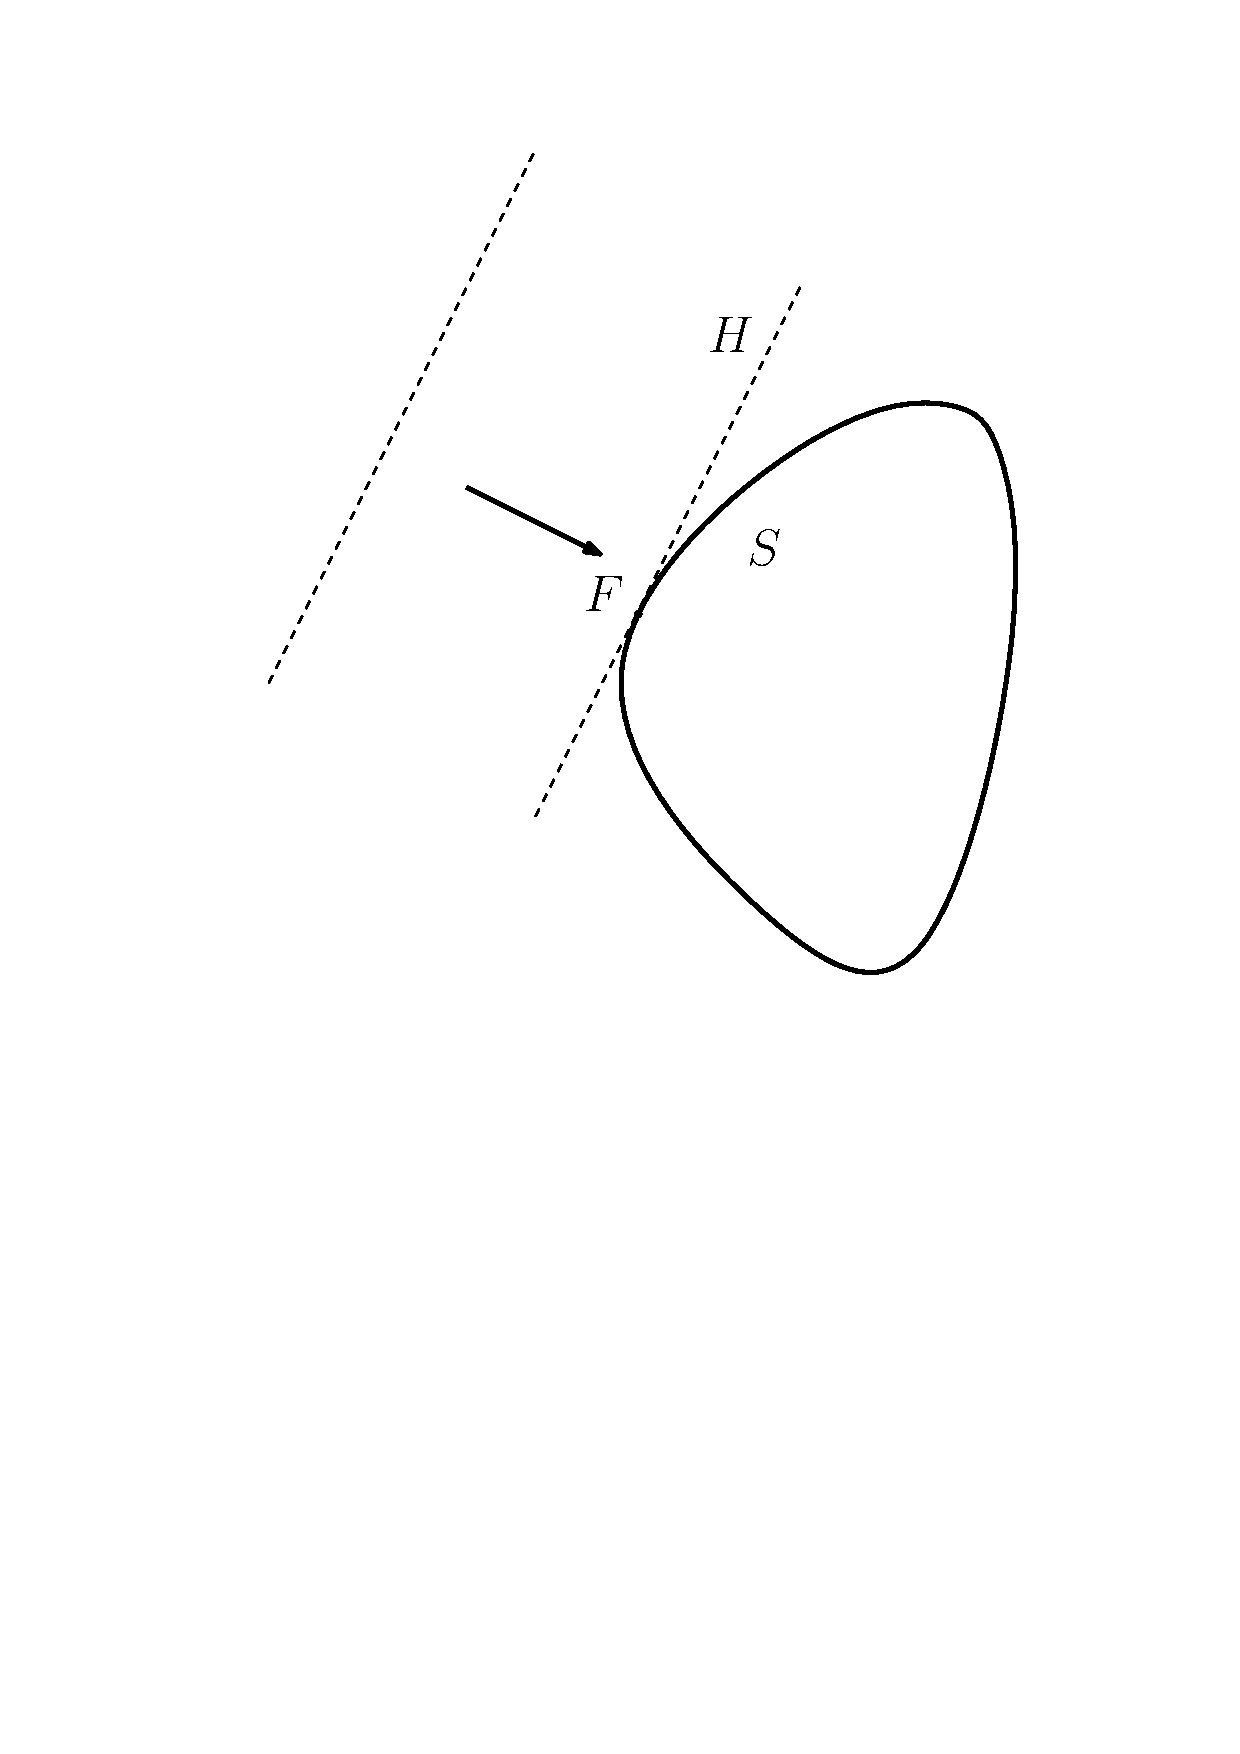
\includegraphics[scale=0.5]{figures/1696891724}

Now, if we let \( H \) be a supporting hyperplane of \( S \) at some point
\( x_{0} \in \operatorname{relbd} S \). Then, \( F = S \cap H \) is an exposed
face, and furthermore, by Lemma \ref{lem:Supporting Hyperplane Theorem (Stronger
variant)}, there exists \( y \in S \) such that \( y \notin H \). Then, \( F
\neq  S \) and therefore \( F \) is a proper face of \( S \).

The other direction, \( x_{0} \in F \) is a proper face of \( S \) implies \(
x_{0} \in \operatorname{relbd} S \), also holds. Let \( A = \operatorname{aff} S
\), then assuming there exists \( x_{0} \in \operatorname{ri } S \cap F \). This
implies that \( B_{A}(x_{0}, \varepsilon) \in S \) for some \( \varepsilon > 0
\), and in this ball we can pick two points \( y \) and \( z \) such that \( x =
\frac{1}{2}(y + z) \). In fact, for every \( y \in B_{A}(x_{0}, \varepsilon) \),
there exists \( z = 2x_{0} - y \) satisfying this property and since \( F \) is a
face, \( y, z \in F \). Hence, \( B_{A}(x_{0}, \varepsilon) \subseteq F \).
Note that \( \dim B_{A}(x_{0}, \varepsilon) = n \), and by Theorem
\ref{thr:No proper faces with full dimensions}, we have a contradiction.

Hence, we have the following lemma.

\begin{lemma}
\label{lem:Points on relative boundary lies on a proper face}
  Let \( S \) be a closed, convex set. Then \( x_{0} \in \operatorname{relbd}
 S \) iff \( x_{0} \) lies on a proper face of \( S \).
\end{lemma}

Now, we will consider some lemmas that will greatly help us in proving the
\textbf{Krein-Milman theorem}.

  \begin{lemma}[Supporting Hyperplane Theorem (Stronger variant)]
  \label{lem:Supporting Hyperplane Theorem (Stronger variant)}

  Let \( C \subseteq \mathbb{R}^{n} \) and \( x_{0} \in \operatorname{relbd} C \).
  Then, there exists hyperplane \( H = \{x, ax = \alpha\}   \) that supports \(
  C\) at \( x_{0} \) such that \( \exists y \in C, ay \neq  \alpha \).
  \end{lemma}

  Theorem \ref{thr:Supporting Hyperplane Theorem} showed that without the last
  condition, \( H \) always exist. This last condition is the only difference
  between the hyperplanes from the basic theorem and this stronger variant.

  Note that this theorem is no longer true for every \( x_{0} \in \partial C \),
  for example considering the segment \( [v_{1}, v_{2}] \) in \( \mathbb{R}^2
  \), its boundary is the whole segment, but one could not construct such a
  supporting hyperplane from a point \( v \) relatively inside the segment, for
  example \( v = \frac{1}{2}(v_{1} + v_{2}) \).

  \begin{proof}[Proof of lemma]
    Let \( A = \operatorname{aff} C, n = \dim_A \). \( n = 0 \) is
    the trivial case, which we will not get into. Consider \( n \ge  1 \).
    
    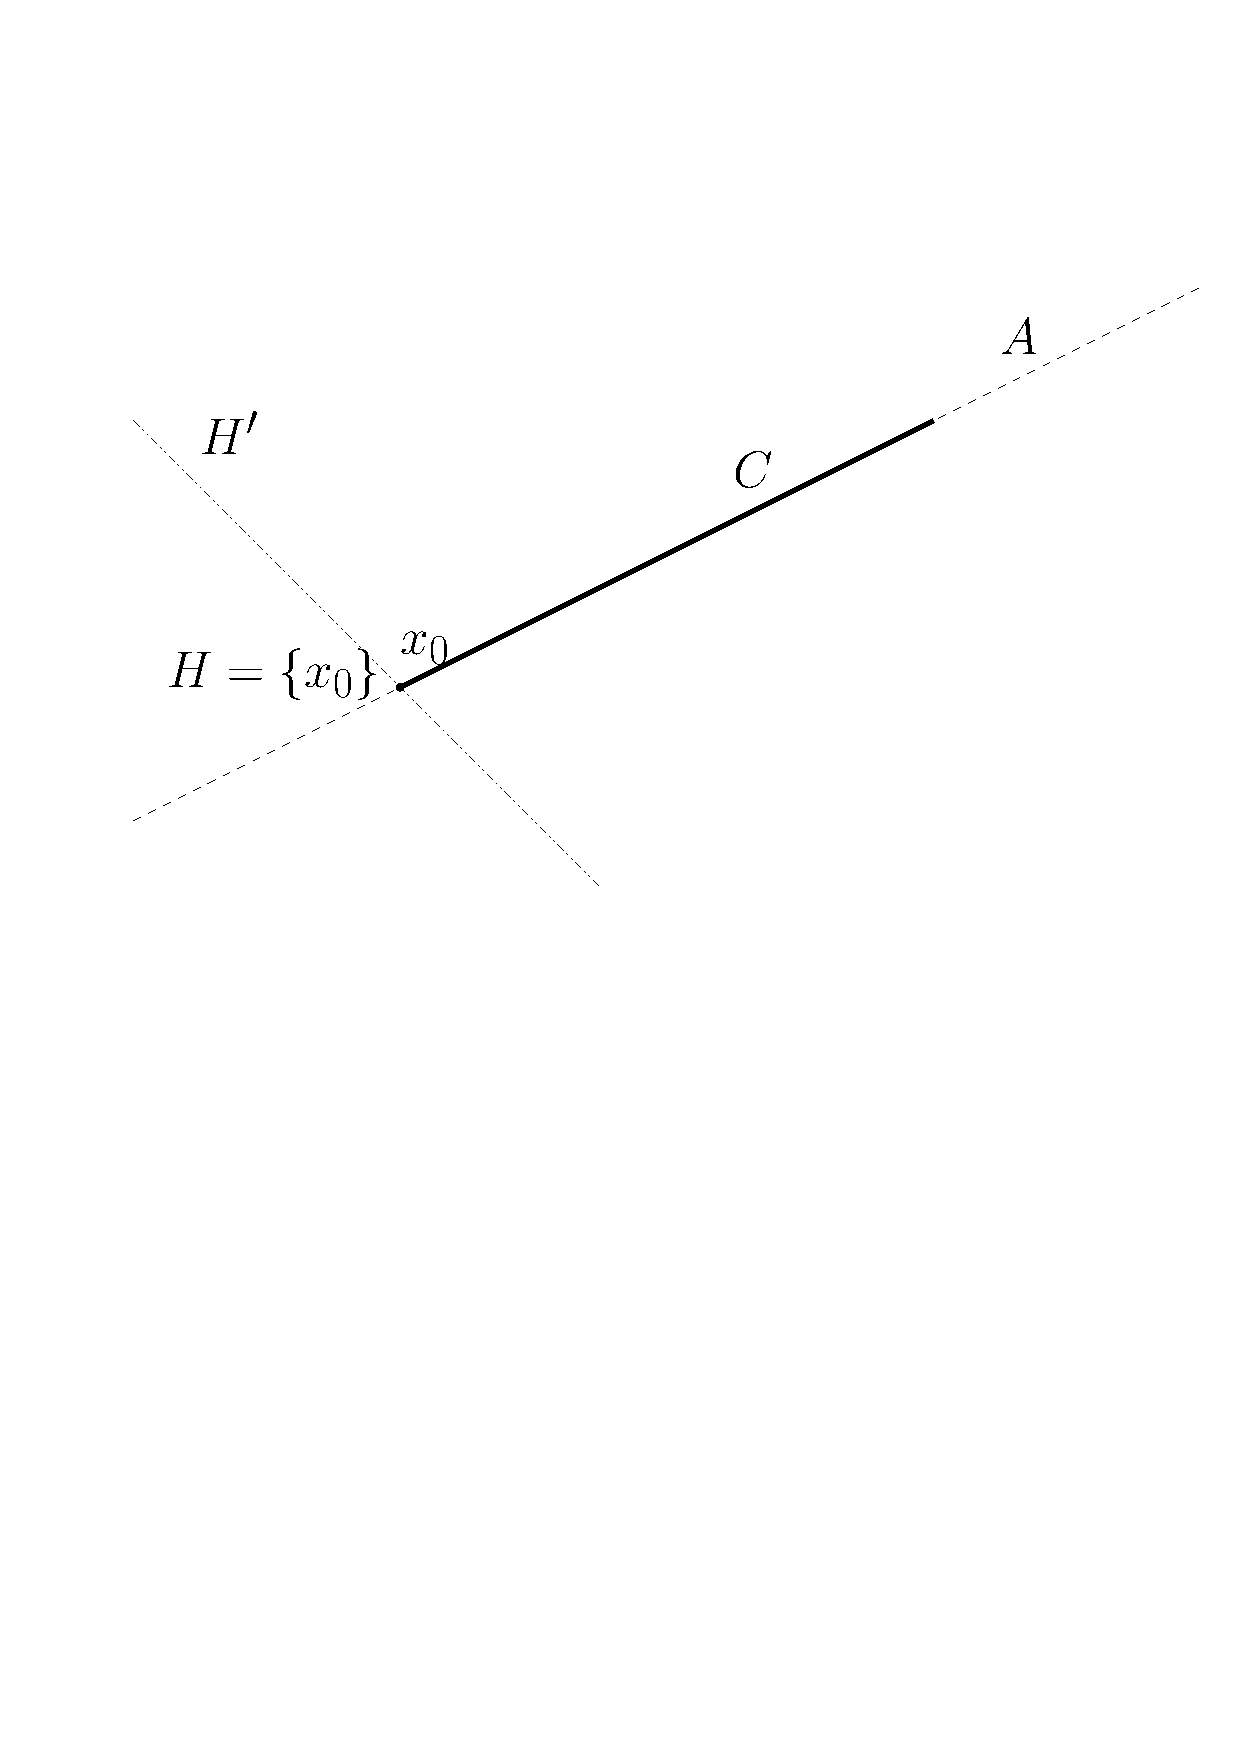
\includegraphics[scale=0.5]{figures/1696827875}

    Then, in the topological space \( (A, \Sigma') \) generated by \( (A, d) \),
    using Theorem \ref{thr:Supporting Hyperplane Theorem}, there exists a
    \( A \)-hyperplane \( H \subseteq A \) that supports \( C \). Then, assuming
    that \( \forall y \in C, y \in H \), which means \( C \subseteq H \). Since
    \( H \) is an affine set and the fact that \( A \) is the minimal affine set
    that contains \( C \), we must have \( A \subseteq H \). Note that \( H
    \subseteq A \), therefore \( A = H \), which means that \(
    \dim A = \operatorname{dim} H \), which could not happen.

    Hence, \( \exists y \in C, y \in H \). Construct a \( \mathbb{R}^{n}
    \)-hyperplane that contains \( H \) and only intersect \( A \) at \( H \),
    we can see that \( H' \) is the hyperplane that satisfies all of the
    conditions we need.
  \end{proof}

\begin{lemma}
\label{lem:xtreme-pt}
  Let \( c \) be a row vector, then the set \( F_{c}(S) = \operatorname{Argmax}
  \{cx, x \in S\}     \), is called an \textbf{exposed face} of \( S \). Then,
  every exposed face is a face.

  An extreme point of a face \( F \) of \( S \) is also an extreme point of \( S
  \).
\end{lemma}

\begin{proof}[Proof of lemma]
  If \( x = \operatorname{lerp}(y,z, w) \in F_{c} \) for some \( y,z \in S \),
  then \( cx = \operatorname{lerp}(cy, cz, w) \le \max \{cy, cz\}   \), which
  means that either \( y \) or \( z \) is a GOS of the problem. WLOG assuming \(
  cx = cy\), then we end up having \( cz = cx \). Therefore, \( y, z \in F_{c}
  \), and \( F_{c} \) is a face of \( S \).

  To prove the second statement, let \( x \) be an extreme point of \( F \).
  Assuming that there exists \( y, z \in S, \lambda \in (0, 1) \) such that \( x =
  \operatorname{lerp}(y, z, \lambda) \), then \( y, z \in F \) because of the
  definition of faces, which leads to a contradiction.
\end{proof}

Returning to the existence theorem, we will define a partial order on \(
\mathcal{A} \), the set of all nonempty exposed faces of \( S \).

If an exposed face \( F \) has one element, then it is the minimal element
in \( \mathcal{A} \),
which means that it could not be "greater" than any other exposed faces,
including other one-element exposed faces.

Otherwise, \( |F| \ge 2 \), we will construct another exposed face that is 
Returning to the existence theorem, denote
\( S_{1} = S \). Then for every \( i \), assuming \( S_{i} \) is a
nonempty face (induction hypothesis) and construct an exposed face \( S_{i+1} \) until we
have found an extreme point of \( S \):
\begin{itemize}
  \item If \( |S_{i}| = 1 \) and \( S_{i} = \{ s\}   \), then \( s \) is an
    extreme point of \( S \).
  \item If \( |S_{i}| \ge  2 \), then pick \( x, y \in S_{i}, x \neq y \). Then,
    consider the hyperplane \( H: ax = \alpha \) separating \( x \) and \( y \),
    i.e. \( ax < \alpha < ay \), which always exists. Then, let \( S_{i+1}
    \coloneqq F_{a}(S_{i}) \subset S_{i} \), which is a nonempty face that is a
    proper subset of \( S_{i} \) (since \( x \notin F_{a} \)).
\end{itemize}

\begin{theorem}[Krein-Milman Theorem]
\label{thr:Krein-Milman Theorem}
  A compact and convex set \( S \) is the convex hull of the set of its extreme
  points.
\end{theorem}

\begin{proof}
  We will use induction on \( n = \dim S \). This is easy to
  verify for \( n = -\infty \) (\( S = \varnothing \)) and \( n = 0 \) (\( S =
  \{x_{0}\}   \)).

  For \( x \in S \), we have two cases:

  \begin{itemize}
  \item If \( x \in \operatorname{relbd} S \), then \( x \) lies on some proper
    face \( F \) of \( S \) with \( \dim F < \operatorname{dim} S
    = n\). Since \( F \) is also compact due to Theorem \ref{thr:Faces and
    extreme points of faces}, \( x \) is a convex combination of the
    extreme points of \( F \), which are also extreme points of \( S \).

  \item If \( x \in \operatorname{ri} S \), consider a line \( L \) passing
    through \( x \) that is contained in \( \operatorname{aff} S \). This line
    intersect \( S \) at some set \( S' \), which is a nonempty (\( x \in S'
    \)), convex (since \( S \) is convex), one-dimensional (since a line is
    one-dimensional). Intuitively (or rigorously using infimums and supremums),
    we can deduce that \( S' \) is a line segment, with the endpoints of \( S'
    \), \( y \) and \( z \) must reside on \( \operatorname{relbd} S \). Then,
    \( y \) and \( z \) are convex combinations of extreme points of \( S \),
    and since \( x \in [y, z] \), \( x \) is a convex combination of \( y \) and
    \( z \), we can see that \( x \), in fact, is a convex combination of the
    extreme points of \( S \).
  \end{itemize}
\end{proof}

% subsection Extreme points and recession directions (end)


\subsection{Convex polyhedra} % (fold)
\label{sub:Convex polyhedra}

\begin{definition}
  A \textbf{convex polyhedron} (plural \textit{convex polyhedra}) \( P \) is
  the intersection of finitely many closed half-spaces.

  A \textbf{convex polytope} is a bounded convex polyhedron.
\end{definition}

Then, one can write \( P \) as \( P = \{x, Ax \ge  b\}   \) for some matrix \( A
\) and row vector \( b \), with the closed half-spaces defining \( P \) being
the half-spaces \( H_{i}: A^{i}x \ge  b^{i} \).

\subsubsection{Extreme points and extreme directions of convex polyhedra} % (fold)
\label{sec:Extreme points and extreme directions of convex polyhedra}

Now, we will take a closer look at the extreme points of a convex polyhedron \(
P\).

\begin{definition}[Tight constraints]
\label{def:Tight constraints}
Let \( P: Ax \le  b \) be a convex polyhedron and \( x \in P \). Then, the set
\[
  \mathbb{I}(x) = \{i \in 1..m, A^{i}x = b^{i}\}  
.\] is called the \textbf{set of tight constraints indices at \( x \)}

In other words, \( \mathbb{I}(x) \) is the maximal multi-index such that \(
A^{I}x = b^{I} \).
\end{definition}

We also denote \( \mathbb{I}(F) \) as the intersection of all \( \mathbb{I}(x), x \in F
\). This will be useful when we look at the tight constraints of faces.

\begin{theorem}
\label{thr:Extreme point of convex polyhedra and matrix rank}
  Let \( P: Ax \le  b, x \in \mathbb{R}^{n} \) be a convex polyhedron.
  Then, \( x \) is an extreme
  point of \( P \) if \( \operatorname{rank} A^{\mathbb{I}(x)} = n \)
\end{theorem}

\begin{proof}
  Denote \( I = \mathbb{I}(x), I^{c} = 1..m \setminus I \).
  Then we can rewrite the conditions of \( x \) into \( A^{I}x = B^{I} \) and \(
  A^{I'}x < B^{I'}\).

  Now, if \( x \) is a convex combination of \( y \) and \( z \) with weight \(
  0 < \lambda < 1\), then 
  \begin{align*}
    b &= A^{I}x\\
      &= A^{I} \operatorname{lerp}(y, z, \lambda)\\
      &= \operatorname{lerp}(A^{I}y, A^{I}z, \lambda)\\
      &\le \operatorname{lerp}(A^{I}x, A^{I}x, \lambda) = A^{I}x = b
  .\end{align*}

  Since \( 0 < \lambda < 1 \), equality only happen when \( A^{I}y = A^{I}z =
  A^{I}x = b \). Hence, if \( \operatorname{rank} A^{I} = n \), the matrix \(
  A^{I} \) is invertible, thus leading to \( y = z = x =(A^{I})^{-1} b \),
  therefore \( x \) is an extreme point of \( P \).

  In the other case, \( \operatorname{rank} A < n \), then there exists \( u \)
  such that \( A^{I}u = 0 \). Consider \( y(\lambda) = x +\lambda u \), then 
  we need to find \( \lambda_{1} > 0 > \lambda_{2} \) such that \(
  y(\lambda_{1}), y(\lambda_{2}) \in P \) and since \( x \) is a strictly convex
  combination of \( y(\lambda_{1}) \) and \( y_{\lambda_{2}} \), \( x \) could
  not be an extreme point.

  Since \( A^{I}y(\lambda) = b^{I} \), we just need \( A^{I^{c}}y(\lambda) \le
  b^{I^{c}} \) to make \( y(\lambda) \in P \). This is trivial since the mapping
  \( f(\lambda) = A^{I^{c}}y(\lambda) \) is linear (and therefore continuous),
  and \( f(0) = A^{I^{c}} x < b^{I^{c}} \).

  Specifically, any \( \lambda \) satisfying \( |\lambda| < \varepsilon \), with
  \( \varepsilon > 0 \) defined as
  \[
    \varepsilon = \min_{\substack{j \in 1..m\\ A^{j}u \neq 0}} \left\{   \frac{b^{j} - A^{j}x}{|A^{j}u|}
  \right\}  
  .\] 
\end{proof}

\begin{corollary}
\label{cor:Finiteness of extreme points in convex polyhedra}
  All convex polyhedra \( P \subseteq \mathbb{R}^{n} \) has finitely many
  extreme points.
\end{corollary}

This is due to the fact that every extreme point of \( P \) corresponds to a set
of tight constraints indices \( \mathbb{I}(x) \), and since there can only be
finitely many such sets (not mentioning the full rank condition), there could
be only finitely many extreme points. An important thing to note is that, the
correspondence between \( x \) and \( \mathbb{I}(x) \) is one-to-one, with \( x
= \left(  A^{\mathbb{I}(x)} \right)^{-1}b\).

Similarly, we also have these analogous results for extreme directions.

\begin{definition}
\label{def:Polyhedral cone}
  A \textbf{polyhedral cone} is a cone that is also a convex polyhedra.
\end{definition}

\begin{theorem}
\label{thr:Recession cone of a convex polyhedra is polyhedral}
  The recession cone of a convex polyhedra \( P: Ax \le  b \) is a polyhedral
  cone \( C: Ax \le 0 \).
\end{theorem}

\begin{theorem}
\label{thr:Extreme directions of convex polyhedra and matrix rank}
  Let \( P: Ax \le  b, d \in \mathbb{R}^{n} \) be a convex polyhedron.
  Then, \( d \) is an extreme
  ray of \( P \) if \( \operatorname{rank} A^{\mathbb{I}(d)} = n - 1 \)
\end{theorem}

\begin{proof}
  By the rank-nullity theorem, \( A^{\mathbb{I}(d)} \) has rank \( n - 1 \) is
  analogous with the fact that the kernel of \( A^{\mathbb{I}(d)} \) is
  one-dimensional. Then, if \( d \) is a convex conical combination of \( d_{1}
  \) and \( d_{2} \), then \( d_{1} \) and \( d_{2} \) are both in this kernel,
  thus making the three vectors \( d_{1} \), \( d_{2} \) and \( d \) lies on the
  same line, which means that \( d \) is an extreme direction.

  The other direction could also be proven similarly to the proof of Theorem
  \ref{thr:Extreme point of convex polyhedra and matrix rank}, by considering
  some vector \(
  u\) linearly independent from \( d \) such that \( A^{\mathbb{I}(d)} = 0 \)
  and consider the function \( d(\lambda) = d + \lambda u \).
\end{proof}

% subsubsection Extreme points and extreme directions of convex polyhedra (end)
\iffalse
\subsubsection{Polar and the Minkowski-Weyl's Theorem} % (fold)
\label{sec:Polar and the Minkowski-Weyl's Theorem}

\begin{definition}[Polar]
\label{def:Polar}
  Let \( V \) be a vector space and \( X \subseteq V \). Then,
  \( X^{\circ} \), called the \textbf{transposed polar} of \( X \), is defined as:
  \[
    X^{\ostar} = \{y \in V^{\star}, yx \le 1, \forall x \in X \}  
  .\], with \( V^{\star} \) denoting the \textbf{dual space} of \( V \).

  If \( V = \mathbb{R}^{n} \) then\footnote{This is an abuse of notation, \(
  V^{\star} \) is supposed to be a set of linear functionals, not matrices.
Also, we will abuse the notation even more, by considering the double dual of a
vector space the same thing as the original vector space (the two spaces are
naturally isomorphic.)}
  \( V^{\star} = \mathbb{R}^{1\times n} \) and
  vice versa, then the \textbf{transpose} operation can be used to convert
  between \( V \) and \( V^{\star} \). Then,
  the transpose of \( X^{\ostar} \) is called the \textbf{polar} of \( X \):
  \[
    X^{\circ} = (X^{\ostar})^{T} = \{x^{T}, x \in X^{\ostar}\}   
  .\] 
\end{definition}

Then, one can see that the polar of a linear space is its orthogonal complement,
For convex cones, the transposed polar can be redefined to \( X^{\circ} = \{y \in
\mathcal{L}(X), yx \le  0, x \in X\}   \).

The polar of an arbitrary (Euclidean) set is a closed and convex set.
since it could be written as intersection of (infinitely many) closed and convex
half-spaces:
\[
  X^{\circ} = \bigcap_{x \in X} \{y \in \mathbb{R}^{n}, y^{T}x \le  1\}  
.\] 

The polar operation can also be applied twice to a set \( X \), resulting in the
set \( (X^{\circ})^{\circ} \), which is not necessarily to be \( X \). In
particular, we have
\[
  (X^{\circ})^{\circ} = \overline{\operatorname{conv} (X \cup  \{0\}  )} 
.\] 

\begin{proof}
  Denote \( X' = (X^{\circ})^{\circ} \), then it is trivial that \( 0 \in X' \)
  and \( X \subseteq X' \). Since \( X' \) is closed and convex, the set \( X''
  = \overline{\operatorname{conv} \{X \cup \{0\}  \}  } \subseteq X' \). Now, we
  just need to prove equality.

  Take \( y \in X''^{c} \), we will prove \( y \in X'^{c} \), which will be what
  we needed. This is equivalent to finding \( z \in X^{\circ} \) such that \( yz
  > 1\). Using Theorem \ref{thr:Hyperplane Separation Theorem}, we find \( H: ax
  = \alpha\) that separates \( \{y\}   \) and \( X'' \), i.e. \( ay > \alpha
  \ge ax, \forall x \in X'' \). Since \( 0 \in X'' \), we have \( \alpha \ge  0
  \).

  If \( \alpha > 0 \), then let \( z = \frac{1}{\alpha} a \), we have \( zx \le 1,
  \forall x \in X\), which means \( z \in X^{\ostar} \). Then, \( zy > 1 \),
  which is a contradiction.

  If \( \alpha = 0 \), then let \( \varepsilon = ay > 0 \), then \( z =
  \frac{2}{\varepsilon}a \) satisfies \( zx \le  1 < 2 = zy, \forall x \in X \),
  which is another contradiction.

  Hence, \( y \) does not exist, and \( X' = X'' \).
\end{proof}
\fi

\subsubsection{Minkowski-Weyl's Theorem} % (fold)
\label{sec:Minkowski-Weyl's Theorem}
Minkowski-Weyl's TheoremAn important property of convex polyhedra is the following theorem.

\begin{theorem}[Minkowski-Weyl's Theorem]
\label{thr:Minkowski-Weyl's Theorem}
  Denote \( \operatorname{conv} V \) as the \textbf{convex hull} of \( V \), \(
  \operatorname{cone} R\) as the convex cone generated by \( R \), \( E(P) \)
  and \( R(P) \) as the set of all extreme points and extreme directions of \( P
  \), respectively. Then
  \begin{itemize}
  \item \textbf{Minkowski's Theorem:}
  \( P \) is a convex polyhedron then
  \( P = \operatorname{conv} E(P) + \operatorname{cone} R(P) \),
  with \( E(P) \) and \( R(P) \) denoting the set of all extreme points and
  extreme directions of \( P \), respectively.
\item \textbf{Weyl's Theorem:}
  If there exists finite sets \( E(P), R(P)  \) such that \( P = \operatorname{conv}
  E(P) + \operatorname{cone} R(P)\), then \( P \) is a convex polyhedron.
  \end{itemize}
\end{theorem}

\begin{proof}
  To prove this theorem, we will try to reduce this problem to the \( b = 0 \)
  case. This case would be proven separately in Theorem
  \ref{thr:Minkowski-Weyl's
  Theorem for Convex Cones}.

  \begin{itemize}
  \item \textbf{Minkowski's Theorem}: Let \( P: Ax \le  b, x \in \mathbb{R}^{n}
    \) Consider the following matrices and
    vectors:
\begin{align*}
  x' &= \begin{bmatrix} x \\ 1 \end{bmatrix} \in \mathbb{R}^{n+1} \\
  A' &= \begin{bmatrix} A & -b \\ -\mathbf{e_{n+1}}^{T} & 0 \end{bmatrix}
  \in \mathbb{R}^{(n + 1) \times  (m + 1)}
\end{align*} (\( \mathbf{e_{n+1}} \) is the \( (n+1) \)-th standard basis
(column) vector).

Then \( Ax \ge b \) if and only if \( A'x' \ge  0 \).

Hence, we will consider the \( (n+1) \)-dimensional polyhedral cone \( C: A'x'
\le  0, x' \in \mathbb{R}^{n+1} \). By Theorem \ref{thr:Minkowski-Weyl's Theorem
for Convex Cones}, \( C = \operatorname{cone} R(C)
\).

    Now take an arbitrary extreme direction \( d' \) of \( C \)
    \[
      d' = \begin{bmatrix} d & z \end{bmatrix} \in \mathbb{R}^{n+1}, \text{ for
      some } d \in \mathbb{R}^{n}, z \in \mathbb{R}
    .\] 

    We have \( A'd' \ge  0 \), which is equivalent to \( Ad - bz \le  0 \) and
    \( z \ge  0 \)

    If \( z = 0 \), then \( Ad \le  b \), which means that \( d \) is an
    recession direction of \( P \). If \( d = \operatorname{lerp}(d_{1}, d_{2},
    \lambda) \) for some \( \lambda \in (0, 1) \) and recession direction \(
    d_{1} \) and \( d_{2} \), we can see that \( d' =
    \operatorname{lerp}(d_{1}', d_{2}', \lambda) \), with \( d'_{i} =
        \begin{bmatrix} d_{i} & 0 \end{bmatrix}^{T}  \), which is a
        contradiction to the fact that \( d' \) is an extreme direction.
    
    If \( z > 0 \), then let \( v = \frac{1}{z} d \), then \( Av \le  b \),
    following a similar logic, we deduce that \( v \) is an extreme point of \(
    P\).

    Denote \( d_{i}' = \begin{bmatrix} d_{i} & z_{i} \end{bmatrix}  \) as
    the \( i \)-th extreme direction of \( C \). Let \( I = \{i, z_{i} > 0\}
    \) and \( I^{c} = \{i, z_{i}  = 0\}   \),
    then \( x' = \begin{bmatrix} x
    & 1\end{bmatrix}  \in C =
    \operatorname{cone} R(C) \) iff there exists \( \lambda \ge 0 \) such that:
    \begin{align*}
      x' &= d_{i}'\lambda^{i}\\
      &= d'_{I}\lambda^{I} + d'_{I^{c}}\lambda^{I^{c}}
    .\end{align*}

    Separating the first \( n \) coordinates and the \( (n+1) \)-th one, we have
    \begin{align*}
      x &= d_{I}\lambda^{I} + d_{I^{c}}\lambda^{I^{c}} \\
      1 &= z_{I}\lambda^{I}
    .\end{align*}

    Substituting \( v_{i} = \frac{1}{z_{i}}d_{i} \in E(P) \), we have
    \begin{align*}
      x &= v_{I}z_{I}\lambda^{I} + d_{I^{c}}\lambda^{I^{c}}\\
      1 &= z_{I}\lambda^{I}
    .\end{align*}

    Finally, denoting \( w_{i} = z_{i}\lambda^{i} \), from the second identity,
    we have the sum of all components of \( w \) is 1, and therefore, we can
    write the above
    expression as \( x = \mathcal{C}(v_{I}, w_{I}) + \mathfrak{C}(d_{I^{c}},
    \lambda^{I^{c}}) \), we have written \( x \) as the sum of a convex
    combination of extreme points \( v_{I} \) and a convex conical combination
    of extreme directions \( d_{I^{c}} \). To prove the other direction, one
    can simply repeat the above logic, but in reverse.

  \item \textbf{Weyl's Theorem:}
    Following the intuition of the above proof, we will consider the set
    \( C = \operatorname{cone} R(C) \), with finite \( R(C) \) given by:
    \begin{align*}
      R(C) &= \left\{ \begin{bmatrix} v \\ 1 \end{bmatrix} , v \in E(P) \right\}
      \cup \left\{ \begin{bmatrix} d \\ 0 \end{bmatrix} , d \in R(P) \right\}  \\
    .\end{align*}
    Then, \( C \) is a polyhedral cone with constraints \( A'x' \le  0 \).
    Assuming
    \begin{align*}
      A' = \begin{bmatrix} A & -b \end{bmatrix}, A \in \mathbb{R}^{(n + 1)
      \times  m}
    ,\end{align*}we have \( P = \{x \in \mathbb{R}^{n}, Ax \le  b\}   \)
  \end{itemize}
\end{proof}

Now, all that's left is to prove Minkowski-Weyl's Theorem for convex cones.

\begin{theorem}[Minkowski-Weyl's Theorem for Convex Cones]
\label{thr:Minkowski-Weyl's Theorem for Convex Cones}
  Let \( P \subseteq \mathbb{R}^{n} \), then the following statements are
  equivalent:

  \begin{enumerate}
  \item \( P \) is a polyhedral cone, i.e. there exists \( A \in \mathbb{R}^{m
    \times  n} \) such that \( P = \{x \in \mathbb{R}^{n}, Ax \le  0\}   \)
  \item \( P \) is a \textit{finitely generated cone}, i.e. there is some matrix
    \( R \) such that \( P = \{x, x = R\lambda, \lambda \ge  0\}   \)
  \end{enumerate}
\end{theorem}

\begin{proof}
  The "\( (2) \implies (1) \)" direction is trivial. One can apply
  Fourier-Motzkin elimination to the linear system of inequalities \( x =
  R\lambda, \lambda \ge 0 \) to eliminate the variables \( \lambda^{1},
  \lambda^{2}, \ldots , \lambda^{k} \) from the system, leaving a system of
  inequalities in the form of \( Ax \le 0 \). Note that no constants were
  generated in the process, hence the \( 0 \) on the RHS.

  Before proceeding, we will introduce a new concept:

  We say that \( (A, R) \) is a \textit{double description pair} (DDP) if
  \( Ax \le  0 \iff \exists \lambda \ge 0, x = R\lambda  \). Then, we will
  proceed to prove that \( (R^{T}, A^{T}) \) is also a DDP.
  \begin{align*}
    &R^{T}y \le 0\\
    &\iff \lambda^{T} R^{T} y \ge 0, \forall  \lambda \ge 0\\
    &\iff (R\lambda)^{T} y \ge 0, \forall  \lambda \ge 0
  .\end{align*}
  Let \( x = R\lambda \), then \( R^{T}y \le 0 \) iff \( x^{T}y \ge 0, \forall
  \lambda \ge 0, x = R\lambda \), or equivalently \( Ax \le  0 \). Then, the
  last statement is equivalent to the statement: \( Ax \le  0 \implies x^{T}y \le  0 \)

  To conclude this proof, we need to use \textbf{Farkas' Lemma}.

  \begin{lemma}[Farkas' Lemma]
  \label{farkas}
    \( ax \ge  0, \forall  x \) s.t. \( Ax \ge  0 \) iff \( a = yA \) for some
    row vector \( y \ge  0 \)
  \end{lemma}

  \begin{proof}[Proof of Farkas' lemma]
    If \( a = yA \), then \( ax = yAx \ge  0, \forall  Ax \ge 0 \).

    If \( ax \ge  0, \forall Ax \ge 0 \) and \( a \neq  yA, \forall  y\ge 0 \),
    then consider the set \( S = \{yA, y \ge 0\}   \). Since \( a \notin S \)
    and \( S \) is closed, using Theorem \ref{thr:hst-closed-pt}, there is a
    hyperplane \( H \) strictly separating \( S^{T} \) and \( \{ a^{T}\}   \).
    Assuming \( H = \{t, x^{T}t \ge  \alpha\}   \) satisfies \( ax  <  \alpha
    \le   \inf Sx \). Note that \( 0 \in Sx \), then \( \alpha \) must be
    non-positive. If \( \alpha < 0 \) and the hyperplane \( H' = \{ t, x^{T}t =
    0\}   \) could not separate the two sets, then there exists some \( t \in S
    \) such that \( tx < 0 \). Then, there exists \( k > 0 \) such that \( t(kx)
    < \alpha\), with \( kx \in S \), which means the original hyperplane also could
    not separate the two sets, which is a contradiction. Hence, the hyperplane
    \( H' \) could separate the two set, i.e. \( ax < 0 \le \inf Sx \). Then,
    we have \( A_{i}x \ge  0 \) for all \( i \), since \( A_{i} =
    A\mathbf{e_{i}} \in S \), with \( \mathbf{e_{i}} \) denoting the \( i \)-th
    standard basis vector, and hence \( Ax \ge 0 \). To conclude, \( ax < 0 \)
    for some \( x \) s.t. \( Ax \ge 0 \), which is another contradiction.
  \end{proof}

Continuing with the proof, we have
\begin{align*}
  &(Ax \le 0 \implies x^{T}y \le 0)\\
  &\iff(Az \ge  0 \implies z^{T}y \ge  0) \text{ (letting \( z = -x \))}\\
  &\iff \exists \lambda \ge 0,  y = \lambda A\\
  &\iff \exists  \lambda' = \lambda^{T} \ge 0, y^{T} = A^{T}\lambda'
.\end{align*}

Hence \( (R^{T}, A^{T}) \) is a DDP.

So to find \( R \), one find do Fourier-Motzkin on \( A^{T} \) to get \( R^{T}
\). Now that \( R \) exists, we have \( C = \{x, Ax \ge 0\} = \{x, \exists
\lambda \ge 0, x = -R\lambda\}  \)

Now, we will prove that \( -R_{i} \) are recession directions of \( C \).
Since \( R_{i} = R\mathbf{e_{i}}, \mathbf{e_{i}} \ge 0 \), \( R_{i} \in P \),
and \( AR_{i} \ge  0 \). Then, for every \( x \in P, t \ge 0 \), we have \( A(x
- tR_{i}) = Ax - tAR_{i} \le  0 \), which means that \( R_{i} \) is a recession
direction of \( C \). Pick columns from \( R \) to form a conical basis of \( R \)'s
column space, then this basis is able to span the recession cone of \( C \), due
to every recession direction \( d \) of \( C \) can be written as \( d =
R\lambda = R'\lambda' \) with some \( \lambda, \lambda' \ge  0 \).
\end{proof}

% subsubsection Minkowski-Weyl's Theorem (end)
\subsubsection{Faces of convex polyhedra} % (fold)
\label{sec:Faces of convex polyhedra}

\begin{theorem}
\label{thr:Basic properties of faces}
  A convex polyhedron only has a finite number of faces. Moreover, all of these
  faces are convex polyhedra.
\end{theorem}

\begin{proof}
  First we will prove the theorem for compact polyhedra.

  Let \( F \) be a face of the compact convex polyhedron \( P \). Then, \( E(F)
  \subseteq E(P) \) and \( F \) is compact. By Theorem \ref{thr:Krein-Milman
  Theorem}, \( F = \operatorname{conv} E(F) \), and by Theorem
  \ref{thr:Minkowski-Weyl's Theorem}, \( F \) is a convex polyhedron. Since
  there are only a finite number of \( E(F) \subseteq E(P) \), there are only
  a finite number of \( F \).

  Back to the general case??????????
\end{proof}

Using this seemingly trivial properties of polyhedral faces, we have the
following theorem.

\begin{theorem}[Face Representation Theorem]
\label{thr:Face Representation Theorem}
  Let \( P \subseteq \mathbb{R}^{n} \) be a convex polyhedron and \( F \subseteq
  P \), then, the following statements are equivalent:

  \begin{enumerate}
    \item \( F \) is a face of \( P \).
    \item \( F \) is an exposed face of \( P \).
    \item There exists multi-index \( I \subseteq 1..m \) such that \( F = \{x
      \in P, A^{I}x = b^{I}\}   \).
  \end{enumerate}
\end{theorem}

\begin{proof}
  \( (3) \implies (1) \) is trivial.

  To prove \( (1) \implies (2) \), let \( x_{0} \in \operatorname{ri} F \). By
  Lemma \ref{lem:Points on relative boundary lies on a proper face}, \( x_{0} \in
  \operatorname{relbd} P \). Let \( H \) be the supporting hyperplane of \( P \)
  at \( x_{0} \), and denote \( G = P \cap H \).

  Then we can see that \( F \subseteq H \) and therefore \( F \subseteq G \).
  Let \( G' \) be the minimal exposed face of \( P \) that contains \( F \),
  induced by the hyperplane \( H: ax = \alpha \). WLOG, assuming \( 
  P\subseteq H^{-}: ax \le  \alpha \).

  We will prove that \( F = G' \). Assuming that this
  is not the case, \( F \) is a proper face of \( G' \) and \( x \in
  \operatorname{relbd} G' \). Therefore, there exists \( H': bx = \beta \),
  the supporting hyperplane of \( G' \) at \( x \). WLOG, assuming \( G'
  \subseteq H'^{-}: bx \le \beta \). Furthermore, using Lemma
  \ref{lem:Supporting Hyperplane Theorem (Stronger variant)}, we can find an \(
  y \in G'\) such that \( by < \beta \).

  Then, \( \forall x \in G', ax \le \alpha, bx \le \beta \). Consider the set \(
  X_{\lambda} = \{x \in P, (\lambda a + b)x = \lambda \alpha + \beta\}  \) for
  some \(  \lambda > 0 \). Then, one can see that \( X_{\lambda} \) is an
  exposed face of \( G' \), and since \( y \notin X_{\lambda} \), it is a proper
  face. To arrive at a contradiction, we will prove that \( X_{\lambda} \)
  contains \( F \) for some \( \lambda > 0 \).

  Rewriting the inequalities of \( X_{\lambda} \), we have \( \lambda(ax
  -\alpha) + (bx - \beta) \le  0 \). For points \( x \in P \) with \( ax -
  \alpha < 0
  \), no matter what \( bx - \beta \) is, the inequality will hold for
  arbitrarily large \( \lambda \). For \( x \in P \) with \( ax - \alpha =0 \),
  we see that \( x \in G' \) and therefore \( bx - \beta \le  0 \), and the
  inequality still holds. Hence, there exists some large \( \lambda > 0 \) such
  that this inequality holds for every \( x \in P \). In particular, here is a
  value for \( \lambda \):
  \[
    \lambda > \max \left\{ 0, \max_{\substack{x\in E(P)\\ax<\alpha}} -\frac{bx
    - \beta}{\alpha - ax}, \max_{\substack{d \in R(P)\\ ad < 0}}  \frac{bd}{-ad}\right\}
  .\] 

  Hence, \( X_{\lambda} \) is an exposed face of \( P \), \( X_{\lambda}
  \subsetneq G' \). Since \( F \subseteq G' \subseteq H: ax = \alpha \) and k

\end{proof}


To conclude, we will take a closer look at the faces of a convex polyhedron \( P
\).

Combining the two finiteness properties, we arrive at the finiteness of faces.

\begin{corollary}
\label{cor:Finiteness of faces in convex polyhedra}
  All convex polyhedra \( P \subseteq \mathbb{R}^{n} \) has finitely many faces.
\end{corollary}

\begin{proof}
Every face, which is a convex polyhedron, corresponds\footnote{This is a
one-to-one correspondence, by Theorem \ref{thr:Minkowski-Weyl's Theorem}, but
since we have left Weyl's theorem unproven, we could not rely on it. Luckily,
relying on Minkowski's theorem alone, we could still establish an injection from
the set of faces to the face's sets of extreme points and extreme directions,
which is sufficient for our purposes.} to
a set of extreme points and extreme directions, which are both finite. Hence,
there could only be finitely many faces for a given convex polyhedron.
\end{proof}


Now, we will consider the faces of a convex polyhedron \( P \).

\begin{theorem}
  Let \( P \) be a convex polyhedron defined by \( P = \{x, Ax \ge  b\}   \).
  
  Denote \( m \) as the number of rows in \( A \) (and \( b \)), then for
  arbitrary \( J \subseteq 1..m \), the set \( F = \{x \in P, A^{J}x = b^{J}\}
  \) is a face of \( P \).
\end{theorem}

\begin{proof}
  Assuming one has \( x \in F \), \( x = \operatorname{lerp}(y, z, \lambda) \)
  with \( \lambda \in (0, 1), y, z \in P \).

  Then, \( b^{J} = A^{J}x = \operatorname{lerp}(A^{J}y, A^{J}z, \lambda) \ge
  \operatorname{lerp}(b^{J}, b^{J}, \lambda) \). Equality only holds if \(
  A^{J}y = A^{J}z = b^{J} \), which means that \( y, z \in F \).
\end{proof}

This result may pose a question: \textit{can all faces \( F \) of \( P \) be
written in the form \( \{x, A^{J}x \ge  b\}  \) for some \( J \)?}

To answer that question, first, we will have to prove the following theorems.

\begin{theorem}[Finiteness of faces in convex polyhedra]
\label{thr:Finiteness of faces in convex polyhedra}
  A convex polyhedron \( P \) has finitely many extreme points and faces.
\end{theorem}

\begin{proof}
  
\end{proof}

\begin{theorem}
\label{thr:Faces and exposed faces in convex polyhedra}
  Every face of a convex polyhedron is an exposed face.
\end{theorem}

\begin{proof}
  Let \( F \) be a face of the convex polyhedron \( P \). Then, if assuming \( F
  \) is a proper face, let \( x \in \operatorname{ri} F \), which is nonempty
  due to Lemma \ref{lem:Nonempty convex set has nonempty interior}. Then,
  consider the supporting hyperplane at \( x \), and the exposed face \( F' \)
  generated by this hyperplane.

  Let \( H: ax = \alpha \) be the supporting hyperplane at \( x \). WLOG
  assuming \( P \subseteq \{x, ax \le  \alpha\}   \), then since \( x \in
  \operatorname{ri} F \), we can write \( x \) as a strictly convex combination
  of an arbitrary \( y \in F \) and some \( z \in F \). Since \( x =
  \operatorname{lerp}(y, z, \lambda) \) and \( ax = \alpha \ge  ay, az \), we
  must have \( ay = az = \alpha \), which means that \( F \subseteq H \) and \(
  F \subseteq F'\).

  Let \( F'' \) be the minimal exposed face that contains \( F \).



\end{proof}

The answer is yes, and it is the result of the following theorem.

\begin{theorem}
\label{thr:Face representation theorem}
  Let \( F \) be a face of the convex polyhedron \( P = \{x, Ax \ge  b\}   \). Then,
  there exists a multi-index \( J \) such that \( F = \{x, A^{J}x = b^{J}\}
  \).
\end{theorem}

\begin{proof}
  Before going on proving the theorem, we will 
  Since \( F \) is a closed convex polyhedron by itself, by
  Theorem \ref{thr:Minkowski-Weyl's Theorem}, \( F =
  \operatorname{conv} E + \operatorname{cone} R \),
  with \( E \) and \( R \) denoting the set of all
  extreme points and extreme directions of \( F \), respectively.

  Assuming that \( F \subseteq F(J) = \{ x \in P, A^{J}x = b^{J}\}   \), then if
  \( i \in J \), we have \( A^{i}x = b^{i} \), which is equivalent to \( A^{i}e
  = b^{i}, \forall e \in E\) and \( Ad = 0, \forall d \in R \). Let \( J \) be
  the set of such indices \( i \), then the theorem is equivalent to proving \(
  F = F(J)\).

  Note that \( F \subseteq F(J) \) due to Theorem \ref{thr:Minkowski-Weyl's
  Theorem}, we just need to prove that \( \nexists x \in F(J) \setminus
  F\). Assuming such \( x \) exists, then
\end{proof}

% subsubsection Faces of convex polyhedra (end)

% subsection Convex polyhedra (end)

% section Convex polyhedra (end)

\section{Existence and properties of solutions of linear programs} % (fold)
\label{sec:Existence and properties of solutions of linear programs}

Firstly, since \( D = \{x\ge 0, Ax \ge  b\}   \) is a convex set (this can be
trivially seen due to the linearity of the convex combination operation) and \(
f(x)=cx\) is a convex (and a concave) function on \( \mathbb{R}^{n} \), then
every (S)LOS of the linear program is a (S)GOS.

The set \( D \) is already closed (why?) and \( f(x) \) is continuous, and hence
the problem will have a GOS if \( D \) is bounded.


% section Existence and properties of solutions of linear programs (end)

% chapter Linear programming (end)
